% ======================================================================
% UNIVERSIDAD PERUANA UNIÓN (UPeU)
% Escuela Profesional de Ingeniería de Sistemas
% Proyecto de Evaluación de Fin de Carrera
% ----------------------------------------------------------------------
% main.tex — Documento maestro (modular, usa \input{} para cada parte)
% Compilar con: pdflatex -> pdflatex (2 veces, para generar el índice)
% ======================================================================

\documentclass[12pt,a4paper]{report}

% ----------------------------------------------------------------------
% 1. CODIFICACIÓN, IDIOMA Y FUENTES
% ----------------------------------------------------------------------
\usepackage[utf8]{inputenc}      % Codificación de entrada UTF-8
\usepackage[T1]{fontenc}         % Salida de fuentes T1 (acentos, "N°", etc.)
\usepackage[spanish,es-noshorthands]{babel} % Español: "Capítulo", guionado, fechas
\usepackage{lmodern}             % Fuente vectorial nítida en PDF

% ----------------------------------------------------------------------
% 2. GEOMETRÍA DE PÁGINA (márgenes estándar de tesis / estilo APA)
% ----------------------------------------------------------------------
\usepackage[a4paper,left=3cm,right=2.5cm,top=2.5cm,bottom=2.5cm,headheight=30pt]{geometry}
\usepackage{setspace}
\onehalfspacing                  % Interlineado 1.5 (estándar en tesis)

% ----------------------------------------------------------------------
% 3. COLOR INSTITUCIONAL UPeU
% ----------------------------------------------------------------------
\usepackage[table]{xcolor}       % [table] habilita \rowcolor/\cellcolor si se requieren
\definecolor{upeublue}{RGB}{0,32,91}   % Azul institucional UPeU
\definecolor{upeugray}{RGB}{88,88,90}  % Gris de apoyo (texto secundario)

% Celda coloreada para el diagrama de Gantt (capítulo 3): \gc marca una semana activa
\newcommand{\gc}{\cellcolor{upeublue!35}}

% ----------------------------------------------------------------------
% 4. IMÁGENES
% ----------------------------------------------------------------------
\usepackage{graphicx}
\graphicspath{{imagenes/}{./}}   % Busca imágenes en /imagenes y en la raíz

% ----------------------------------------------------------------------
% 5. TABLAS PROFESIONALES (booktabs + tabularx, sin bordes verticales)
% ----------------------------------------------------------------------
\usepackage{array}
\usepackage{booktabs}
\usepackage{tabularx}
\usepackage{longtable}
\usepackage{caption}
\captionsetup{
  labelfont={bf,color=upeublue},
  font=small,
  justification=justified,
  singlelinecheck=false
}
\renewcommand{\arraystretch}{1.25}

% Columnas reutilizables para tabularx: ancho fijo con alineación fija
\newcolumntype{L}[1]{>{\raggedright\arraybackslash}p{#1}}
\newcolumntype{C}[1]{>{\centering\arraybackslash}p{#1}}
\newcolumntype{R}[1]{>{\raggedleft\arraybackslash}p{#1}}

% ----------------------------------------------------------------------
% 6. LISTAS Y RECUADROS DESTACADOS (cajas de nota / conclusión tipo UPeU)
% ----------------------------------------------------------------------
\usepackage{enumitem}
\setlist{itemsep=2pt, topsep=4pt, parsep=0pt}

\usepackage[most]{tcolorbox}
\tcbuselibrary{breakable,skins}

% Caja destacada institucional: \begin{upeubox}{Título} ... \end{upeubox}
\newtcolorbox{upeubox}[1]{
  enhanced,
  breakable,
  colback=upeublue!5,
  colframe=upeublue,
  colbacktitle=upeublue,
  coltitle=white,
  fonttitle=\bfseries,
  title={#1},
  boxrule=0.6pt,
  arc=1.5pt,
  left=8pt, right=8pt, top=6pt, bottom=6pt,
  before skip=10pt, after skip=10pt
}

% ----------------------------------------------------------------------
% 7. TÍTULOS DE CAPÍTULO / SECCIÓN CON COLOR INSTITUCIONAL
% ----------------------------------------------------------------------
\usepackage{titlesec}

% Portada de PARTE = una LÍNEA de la evaluación (CE01 / CE02 / CE03)
\titleformat{\part}[display]
  {\normalfont\bfseries\color{upeublue}\filcenter}
  {\Large\MakeUppercase{\partname}~\thepart}
  {14pt}
  {\titlerule[1.2pt]\vspace{12pt}\Huge}
\titlespacing*{\part}{0pt}{60pt}{40pt}

\titleformat{\chapter}[display]
  {\normalfont\bfseries\huge\color{upeublue}}
  {\filright\Large\MakeUppercase{\chaptertitlename}~\thechapter}
  {10pt}
  {\titlerule[1pt]\vspace{10pt}\Huge}
\titlespacing*{\chapter}{0pt}{0pt}{30pt}

\titleformat{\section}
  {\normalfont\Large\bfseries\color{upeublue}}{\thesection}{0.8em}{}
\titlespacing*{\section}{0pt}{18pt}{8pt}

\titleformat{\subsection}
  {\normalfont\large\bfseries\color{upeublue!85!black}}{\thesubsection}{0.8em}{}
\titlespacing*{\subsection}{0pt}{14pt}{6pt}

\titleformat{\subsubsection}
  {\normalfont\normalsize\bfseries\itshape\color{upeugray}}{\thesubsubsection}{0.8em}{}
\titlespacing*{\subsubsection}{0pt}{12pt}{4pt}

% ----------------------------------------------------------------------
% 8. ENCABEZADOS Y PIES DE PÁGINA
% ----------------------------------------------------------------------
\usepackage{fancyhdr}
\pagestyle{fancy}
\fancyhf{}
\renewcommand{\headrulewidth}{0.4pt}
\renewcommand{\footrulewidth}{0pt}

% La marca de encabezado muestra únicamente "Capítulo N" (sin título ni secciones)
\renewcommand{\chaptermark}[1]{\markboth{\chaptername\ \thechapter}{}}

% Izquierda: logo WISP en pequeño · Derecha: "Capítulo N"
\fancyhead[L]{\raisebox{-0.35\height}{
\includegraphics[height=7mm]{imagenes/Wisp.png}}}
\fancyhead[R]{\small\itshape\color{upeugray}\nouppercase{\leftmark}}
\fancyfoot[C]{\small\thepage}

\fancypagestyle{plain}{ % Estilo de la primera página de cada capítulo
  \fancyhf{}
  \fancyfoot[C]{\small\thepage}
  \renewcommand{\headrulewidth}{0pt}
}

% ----------------------------------------------------------------------
% 9. HIPERVÍNCULOS (se carga al final del preámbulo, según buenas prácticas)
% ----------------------------------------------------------------------
\usepackage{hyperref}
\hypersetup{
  colorlinks   = true,
  linkcolor    = upeublue,
  citecolor    = upeublue,
  urlcolor     = upeublue,
  filecolor    = upeublue,
  pdftitle     = {Sistema de Gestión Integral para ISP de Fibra Óptica Multi-Zona},
  pdfauthor    = {Universidad Peruana Unión - Escuela Profesional de Ingeniería de Sistemas},
  pdfsubject   = {Proyecto de Evaluación de Fin de Carrera - Línea GTI},
  pdfkeywords  = {UPeU, GTI, WISP, Fibra Óptica, ISP, Ingeniería de Sistemas},
  bookmarksnumbered = true,
  bookmarksopen     = true
}
\usepackage[capitalise,spanish]{cleveref} % \Cref{} / \cref{} para referencias cruzadas

% ======================================================================
% DOCUMENTO
% ======================================================================
\begin{document}

% --------------------------- PÁGINAS PRELIMINARES ---------------------
\pagenumbering{roman}

% ======================================================================
% caratula.tex — Portada / carátula institucional UPeU
% ======================================================================
\begin{titlepage}
\begin{center}

% ---------- LOGO INSTITUCIONAL (opcional) ----------
% Si existe imagenes/logo_upeu.png se muestra; si no, la carátula sigue limpia.
\IfFileExists{imagenes/logo_upeu.png}{%
  
\includegraphics[width=0.28\textwidth]{imagenes/logo_upeu.png}\par
  \vspace{0.6cm}
}{}

% ---------- INSTITUCIÓN ----------
{\Large\bfseries UNIVERSIDAD PERUANA UNIÓN\par}
\vspace{0.3cm}
{\large Escuela Profesional de Ingeniería de Sistemas\par}

\vspace{1.3cm}



% ---------- TÍTULO DEL PROYECTO ----------
{\color{upeublue}\bfseries\LARGE
Modernización Operativa y Tecnológica en Telecomunicaciones\\[4pt]
Ecosistema Multi-Zona para WISP\par}

\vspace{0.5cm}
{\normalsize\bfseries\color{upeugray}%
LÍNEA: GESTIÓN DE TECNOLOGÍAS DE INFORMACIÓN (GTI)\par}

\vspace{1.2cm}

% ---------- LOGO DEL CASO DE ESTUDIO (WISP) ----------

\includegraphics[width=0.48\textwidth]{imagenes/Wisp.png}\par
\vspace{0.4cm}
{\large Caso de estudio:\par}
{\Large\bfseries WISP Ingeniería en Redes y Telecomunicaciones\par}

\vfill

% ---------- INTEGRANTES ----------
{\large\bfseries Integrantes\par}
\vspace{0.35cm}
{\normalsize
\renewcommand{\arraystretch}{1.35}
\begin{tabular}{@{}l l@{}}
Cabana Sulca, Cristian & \textbf{202212416} \\
Montes Mamani, Andrés Lino & \textbf{202212423} \\
Fernández Sánchez, Jean Piero & \textbf{202212439} \\
Mamani Mamani, Alessandro Pastor & \textbf{202212452} \\
\end{tabular}\par}

\vfill

% ---------- LUGAR Y AÑO ----------
{\large Juliaca, Puno --- Perú\par}
{\large 2026\par}

\end{center}
\end{titlepage}


\tableofcontents
\listoftables
\listoffigures

\clearpage
\pagenumbering{arabic}

% --------------------------- CUERPO DEL DOCUMENTO ----------------------
% El documento integra las TRES líneas de la evaluación de perfil de proyecto de
% egreso. Cada línea es una \part{}; sus entregables son los capítulos internos.
% La numeración de capítulos es continua a lo largo de todo el documento.

% ====================== LÍNEA CE01 · GESTIÓN DE TI (GTI) ======================
\part{Línea CE01 — Gestión de Tecnologías de Información}
% ======================================================================
% capitulos/capitulo1.tex
% ----------------------------------------------------------------------
% ENTREGABLE 1 — Diagnóstico Organizacional y Alineamiento Estratégico
% Empresa caso de estudio: WISP Ingeniería en Redes y Telecomunicaciones
% Contenido trasladado desde Entregable1_GTI_WISP.docx
% ======================================================================
\chapter{Diagnóstico Organizacional y Alineamiento Estratégico}
\label{chap:diagnostico}

% ----------------------------------------------------------------------
% Descripción del producto (introducción del capítulo)
% ----------------------------------------------------------------------
El presente documento constituye el Entregable~1 de la línea de Gestión de
Tecnologías de Información (GTI) del Proyecto de Evaluación de Fin de Carrera.
Corresponde a un análisis estructurado de la situación actual de la empresa
WISP Ingeniería en Redes y Telecomunicaciones, orientado a identificar sus
brechas estratégicas, operativas y tecnológicas.

El análisis incluye la evaluación del contexto interno y externo de la
organización, el grado de madurez en tecnologías de información y la coherencia
entre los objetivos estratégicos institucionales y las capacidades digitales
existentes. Este componente fundamenta la necesidad del proyecto y garantiza su
alineamiento con el plan estratégico organizacional y el plan estratégico de TI,
sentando las bases para el desarrollo de una solución tecnológica integral que
abarca las líneas de Gestión de TI, Ingeniería de Software e Infraestructura
Tecnológica.

\begin{upeubox}{Alcance del documento}
Este entregable cubre los cuatro componentes exigidos por la rúbrica:
(1.1)~Contexto Organizacional, (1.2)~Análisis Estratégico,
(1.3)~Diagnóstico Digital~/~TI y (1.4)~Identificación del Problema. Los
resultados de este diagnóstico alimentan directamente el Business Case, el Plan
de Gestión del Proyecto y el diseño de la solución técnica integrada.
\end{upeubox}

% ======================================================================
\section{Contexto Organizacional}
\label{sec:contexto}

\subsection{Descripción del sector y entorno competitivo}

WISP Ingeniería en Redes y Telecomunicaciones (en adelante, WISP) es una empresa
peruana del sector de telecomunicaciones, especializada en la provisión del
servicio de acceso a internet mediante red de fibra óptica (FTTH~--~\textit{Fiber
To The Home}) y televisión digital en zonas rurales y semi-rurales de la región
Puno. La empresa opera en un segmento de mercado caracterizado por una baja
penetración de servicios de conectividad de banda ancha y una limitada presencia
de los operadores de telecomunicaciones de escala nacional.

El sector de telecomunicaciones en el Perú es un mercado regulado por el
Organismo Supervisor de Inversión Privada en Telecomunicaciones (OSIPTEL) y el
Ministerio de Transportes y Comunicaciones (MTC). En las grandes ciudades de la
región, como Puno y Juliaca, la competencia es intensa y está conformada tanto
por operadores nacionales ---Movistar, Claro, Entel y WOW--- como por operadores
locales de fibra óptica de creciente presencia, entre los que destacan Fibramax,
WiwiTel, FiberUltra y otros proveedores regionales. Estos actores concentran su
inversión en las zonas urbanas de alta densidad poblacional, donde la
rentabilidad por kilómetro de red desplegada es mayor.

Sin embargo, en los distritos rurales alejados donde opera WISP, la presencia de
estos operadores es marginal o inexistente, debido a la baja densidad
poblacional, la dispersión geográfica y la complejidad logística que implica el
despliegue de infraestructura de fibra en dichas zonas. Esta característica del
mercado configura una ventaja competitiva estructural para WISP: la empresa
atiende un mercado desatendido por los grandes operadores y por la mayoría de los
ISP locales, contribuyendo activamente a la reducción de la brecha digital en la
región Puno. WISP ya cuenta con infraestructura de fibra óptica desplegada y
operativa en trece~(13) zonas distribuidas en distintas provincias de la región.

\subsubsection{Zonas de cobertura y modalidad de servicio}

WISP brinda el servicio de internet por fibra óptica en las siguientes zonas de
la región Puno:

\begin{center}
\captionof{table}{Zonas de cobertura de fibra óptica de WISP en la región Puno.}
\label{tab:zonas}
\begin{tabularx}{\textwidth}{C{1.1cm} X C{1.1cm} X}
\toprule
\textbf{N°} & \textbf{Zona / Distrito} & \textbf{N°} & \textbf{Zona / Distrito} \\
\midrule
1 & Cabana        & 8  & Mañazo  \\
2 & Cabanilla     & 9  & Muñani  \\
3 & Cabanillas    & 10 & Ñuñoa   \\
4 & Capachica     & 11 & Pucara  \\
5 & Choquehuanca  & 12 & Sucasco \\
6 & Domingo       & 13 & Vilque  \\
7 & Huata         &    &         \\
\bottomrule
\end{tabularx}
\end{center}

\begin{upeubox}{Nota sobre el entorno competitivo (dato de campo)}
Debe distinguirse entre el mercado urbano y el rural, porque la competencia que
enfrenta WISP es radicalmente distinta en cada uno:
\begin{itemize}[leftmargin=1.4em]
  \item \textbf{En las ciudades (Puno y Juliaca):} el mercado es altamente
  competitivo, con operadores nacionales (Movistar, Claro, Entel, WOW) y locales
  de fibra (Fibramax, WiwiTel, FiberUltra, entre otros). WISP no compite
  directamente en este segmento.
  \item \textbf{En los distritos rurales (zona de operación de WISP):} el único
  competidor con fibra óptica es FiberUltra, y solo en dos distritos: Cabanillas
  y Mañazo. En el resto de zonas ---e incluso en esos dos distritos--- la
  competencia se limita a pequeños proveedores de internet inalámbrico
  (radioenlaces), de menor estabilidad y capacidad que la fibra. En la mayoría de
  sus zonas, WISP es el único proveedor de fibra óptica, una posición de ventaja
  competitiva difícil de replicar en el corto plazo.
\end{itemize}
\end{upeubox}

\subsection{Estructura organizacional}

WISP opera bajo una estructura organizacional funcional y de tamaño reducido,
característica de una micro/pequeña empresa (MYPE) del sector tecnológico. La toma
de decisiones está centralizada en la administración, y las áreas operativas
(técnica y comercial) se despliegan sobre las trece zonas de cobertura. La
estructura actual del personal es la siguiente:

\begin{center}
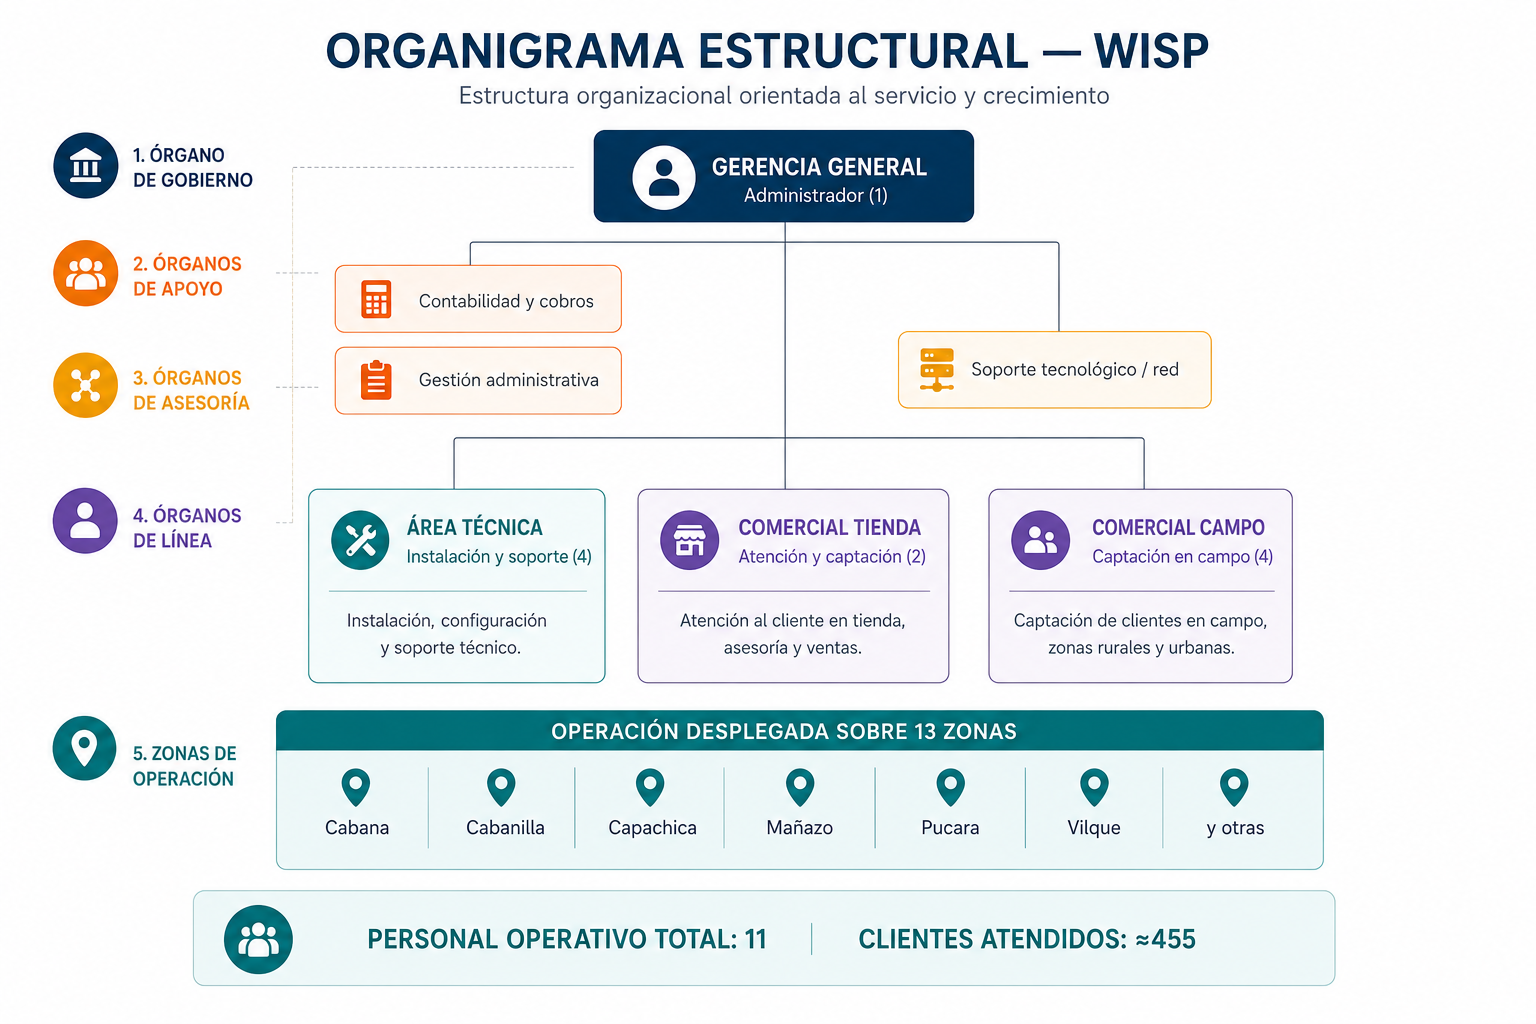
\includegraphics[width=\textwidth]{organigrama.png}
\captionof{figure}{Estructura del personal de WISP por área y responsabilidades.}
\label{fig:estructura}
\end{center}

\begin{upeubox}{Observación estructural crítica}
Un solo administrador concentra la gestión de aproximadamente 455 clientes
distribuidos en 13 zonas geográficamente dispersas. Esta alta concentración de
responsabilidades en una sola persona constituye un \textbf{punto único de falla}
operativo y una limitación severa para el crecimiento, aspecto que se profundiza
en el diagnóstico de TI (Sección~\ref{sec:diagnostico}) y en la identificación
del problema (Sección~\ref{sec:problema}).
\end{upeubox}

\subsection{Cadena de valor}

Siguiendo el modelo de Michael Porter, la cadena de valor de WISP descompone la
empresa en sus actividades constitutivas para identificar las fuentes de ventaja
competitiva. Las actividades se dividen en primarias (directamente involucradas
en la creación y entrega del servicio al cliente) y de apoyo (que respaldan a las
primarias). El margen resulta de la diferencia entre el valor que el cliente está
dispuesto a pagar y el costo de desarrollar dichas actividades.

El análisis revela un hallazgo central: el flujo de información atraviesa
transversalmente toda la cadena, y su gestión deficiente ---actualmente basada en
WhatsApp, papel y un sistema heredado--- erosiona el margen al elevar los costos
operativos y de coordinación en cada eslabón.

\begin{center}
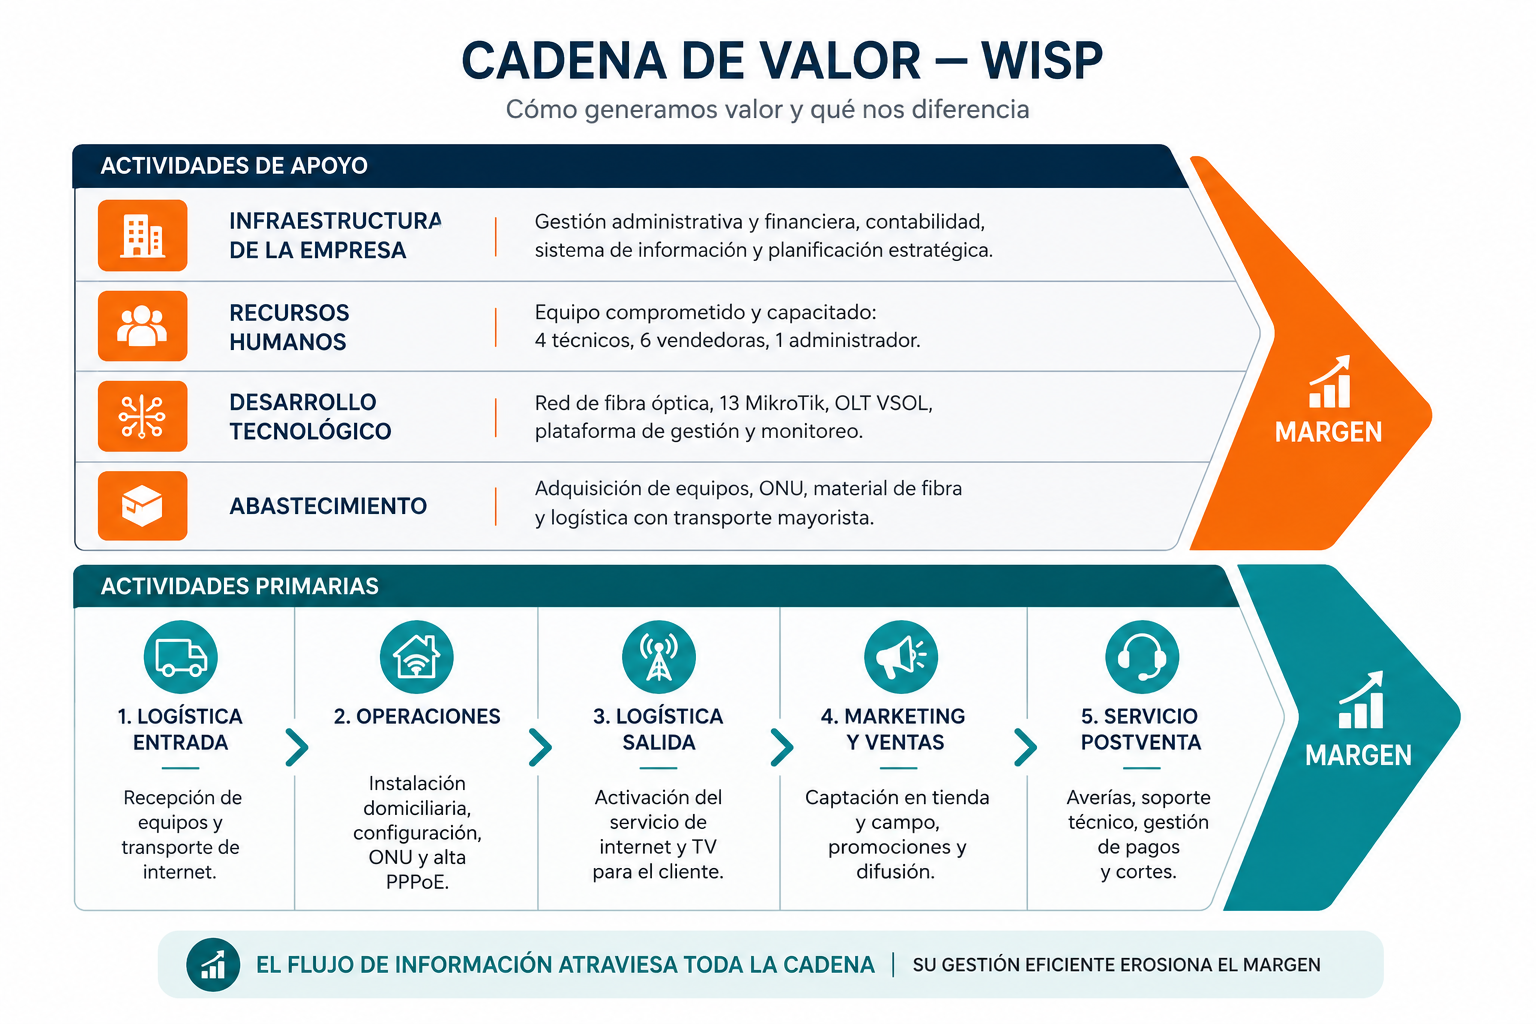
\includegraphics[width=\textwidth]{cadena_de_valor.png}
\captionof{figure}{Cadena de valor de WISP según el modelo de Michael Porter.}
\label{fig:cadena-valor}
\end{center}

\begin{upeubox}{Diagnóstico de la cadena de valor}
La ventaja competitiva de WISP se sustenta hoy en su Desarrollo Tecnológico de red
(infraestructura de fibra madura) y en su cercanía al cliente en Marketing/Ventas
y Servicio postventa. Sin embargo, el margen se ve comprometido porque la
Infraestructura de la empresa (sistemas de información y gestión) opera en un nivel
deficiente que encarece y ralentiza todas las actividades primarias. El proyecto
interviene precisamente sobre esta actividad de apoyo transversal para liberar el
potencial de toda la cadena.
\end{upeubox}

\subsection{Mapa de stakeholders}

Se identifican los grupos de interés (\textit{stakeholders}) internos y externos
que se relacionan con la operación de WISP y que serán impactados directa o
indirectamente por el proyecto de transformación tecnológica. Se clasifican según
su naturaleza, su rol y su nivel de influencia e interés en el proyecto.

\begin{center}
\captionof{table}{Mapa de stakeholders del proyecto.}
\label{tab:stakeholders}
\begin{tabularx}{\textwidth}{L{2.9cm} C{1.4cm} X C{1.5cm} C{1.3cm}}
\toprule
\textbf{Stakeholder} & \textbf{Tipo} & \textbf{Rol / Interés principal} & \textbf{Influencia} & \textbf{Interés} \\
\midrule
Administrador / Gerente & Interno &
Decisor. Busca control total de la operación y eficiencia administrativa. & Alta & Alto \\
Técnicos (4) & Interno &
Operativo. Requieren herramientas que simplifiquen instalaciones y registro de averías. & Media & Alto \\
Vendedoras tienda (2) & Interno &
Comercial. Registro rápido y validación de prospectos. & Media & Alto \\
Vendedoras campo (4) & Interno &
Comercial. Necesitan app móvil para registrar clientes sin papel ni WhatsApp. & Media & Alto \\
Clientes finales ($\approx$455) & Externo &
Usuario. Buscan servicio estable, atención rápida y comunicación clara. & Baja & Alto \\
Proveedor mayorista de internet & Externo &
Soporte. Provee el transporte de última milla; interesa continuidad. & Alta & Medio \\
Competidores (FiberUltra, ISP inalámbricos) & Externo &
Amenaza. Compiten por captación de clientes en zonas compartidas. & Media & Bajo \\
Entes reguladores (OSIPTEL, MTC) & Externo &
Regulación. Supervisan cumplimiento normativo del servicio. & Alta & Bajo \\
\bottomrule
\end{tabularx}
\end{center}

\begin{upeubox}{Priorización de stakeholders (matriz Poder--Interés)}
Los stakeholders de mayor prioridad para el proyecto (alta influencia $+$ alto
interés) son el administrador y, en su conjunto, el personal operativo (técnicos y
vendedoras). Estos serán los usuarios directos del sistema y su adopción
determinará el éxito de la iniciativa. Los clientes finales, aunque de baja
influencia directa, tienen alto interés porque percibirán la mejora en la calidad
y rapidez del servicio.
\end{upeubox}

% ======================================================================
\section{Análisis Estratégico}
\label{sec:estrategico}

El análisis estratégico establece el marco de referencia sobre el cual se sustenta
la necesidad del proyecto. Se formaliza la misión, visión y objetivos estratégicos
de WISP, se evalúa su situación interna y externa mediante el análisis FODA, se
complementa con un análisis PESTEL del macroentorno y se determinan los factores
críticos de éxito.

\subsection{Misión, visión y objetivos estratégicos}

\begin{upeubox}{Justificación de la propuesta}
Dado que WISP, por ser una MYPE de estructura reducida y decisiones
centralizadas, no contaba con una misión y visión formalmente declaradas,
este documento las formula por primera vez aplicando el marco teórico del
planeamiento estratégico.
\end{upeubox}

\begin{upeubox}{Misión (propuesta formalizada)}
"Proveer acceso a internet de alta velocidad por fibra óptica y televisión digital,
con estándares de calidad, estabilidad y trazabilidad, a las familias y negocios
de las zonas de la región Puno, sustentados en infraestructura propia,
un servicio técnico cercano y un modelo de gestión eficiente que garantiza
continuidad y precios accesibles."
\end{upeubox}

La \textbf{misión} responde a las tres preguntas fundamentales del modelo de
formulación estratégica: \emph{qué} necesidad satisface WISP (acceso a internet
de calidad en zonas desatendidas), \emph{cómo} la satisface (mediante
infraestructura propia de fibra óptica y atención cercana) y \emph{a quiénes}
atiende (las familias y negocios de las comunidades de la región Puno). Su
contenido no es arbitrario: se deriva del diagnóstico organizacional (FODA,
cadena de valor) y de los valores institucionales de la empresa.

\begin{upeubox}{Visión (propuesta formalizada)}
"Al 2030, ser el proveedor líder de internet por fibra óptica de Puno,
llevando conectividad de calidad y nuevas oportunidades a las zonas donde otros no llegan."
\end{upeubox}

La \textbf{visión} cumple las cinco características que exige el marco teórico:
es \emph{inspiradora} (proyecta el propósito de llegar donde otros no llegan),
\emph{clara y concisa} (con un horizonte definido al 2030), \emph{ambiciosa
pero realista} (el liderazgo en fibra es una posición que WISP ya casi
ocupa), \emph{relevante y sostenible} (alineada con los objetivos estratégicos
de expansión y escalabilidad) y \emph{flexible y adaptativa} (no se limita a un
número fijo de zonas, permitiendo el crecimiento futuro).

En conjunto, misión y visión quedan alineadas entre sí y con los valores
institucionales, garantizando la coherencia estratégica que el planeamiento
requiere.

\subsubsection{Valores institucionales}

Los valores constituyen la brújula ética que orienta el comportamiento y las
decisiones de WISP, y sirven de base a su cultura organizacional:

\begin{center}
\captionof{table}{Valores institucionales de WISP.}
\label{tab:valores}
\begin{tabularx}{\textwidth}{L{3.4cm} X}
\toprule
\textbf{Valor} & \textbf{Significado en WISP} \\
\midrule
Cercanía & Atención personalizada y trato directo con el cliente rural, entendiendo su realidad y necesidades. \\
Compromiso social & Vocación de cerrar la brecha digital y llevar conectividad a zonas que otros operadores no atienden. \\
Calidad y confiabilidad & Provisión de un servicio estable, con infraestructura de fibra óptica robusta y soporte técnico propio. \\
Innovación & Adopción de tecnología para mejorar continuamente la operación y la experiencia del cliente. \\
Integridad & Transparencia en el cobro, en los contratos y en la relación con clientes y colaboradores. \\
\bottomrule
\end{tabularx}
\end{center}

A partir de la misión, visión y valores, se derivan los siguientes objetivos
estratégicos institucionales:

\begin{center}
\captionof{table}{Objetivos estratégicos institucionales de WISP.}
\label{tab:objetivos}
\begin{tabularx}{\textwidth}{C{1.4cm} X L{2.3cm}}
\toprule
\textbf{Código} & \textbf{Objetivo estratégico} & \textbf{Perspectiva} \\
\midrule
OE-01 & Expandir la cobertura de fibra óptica a nuevos distritos de la región Puno actualmente desatendidos. & Crecimiento \\
OE-02 & Mejorar la eficiencia operativa mediante la digitalización y automatización de los procesos de captación, instalación, soporte y gestión de clientes. & Procesos \\
OE-03 & Incrementar la satisfacción y retención de clientes a través de un servicio estable y una atención más rápida y trazable. & Cliente \\
OE-04 & Fortalecer el control administrativo y financiero, reduciendo la morosidad y la dependencia de procesos manuales. & Financiera \\
OE-05 & Consolidar una plataforma tecnológica escalable que soporte el crecimiento de la empresa sin incrementar proporcionalmente la carga administrativa. & Tecnología \\
\bottomrule
\end{tabularx}
\end{center}

\subsection{Análisis FODA}

El análisis FODA sintetiza los factores internos (fortalezas y debilidades) y
externos (oportunidades y amenazas) que condicionan la posición estratégica de
WISP. Se presenta primero en forma de matriz y luego se detalla cada cuadrante.

\begin{center}
\captionof{table}{Matriz FODA de WISP.}
\label{tab:foda}
\begin{tabularx}{\textwidth}{X X}
\toprule
\rowcolor{upeublue!10}
\textbf{FORTALEZAS (F)} & \textbf{DEBILIDADES (D)} \\
\midrule
\begin{itemize}[leftmargin=1.4em,nosep]
  \item F1. Infraestructura propia de fibra óptica en 13 zonas.
  \item F2. Único proveedor de fibra en la mayoría de sus zonas.
  \item F3. Servicio técnico propio (4 técnicos).
  \item F4. Fuerza de ventas en campo desplegada por zonas.
  \item F5. Portafolio de planes con TV integrada (\textit{triple play}).
  \item F6. Conocimiento del mercado rural y cercanía con el cliente.
\end{itemize}
&
\begin{itemize}[leftmargin=1.4em,nosep]
  \item D1. Sistema de gestión heredado (PHP) lento y mal diseñado.
  \item D2. Operación dependiente de WhatsApp, sin trazabilidad.
  \item D3. Sin aplicación móvil para técnicos ni vendedoras.
  \item D4. Un solo administrador para 13 zonas (punto único de falla).
  \item D5. Sin historial técnico por cliente (caja NAP, borne, ONU).
  \item D6. Inconsistencia de datos entre MikroTiks y planes comerciales.
\end{itemize}
\\
\midrule
\rowcolor{upeublue!10}
\textbf{OPORTUNIDADES (O)} & \textbf{AMENAZAS (A)} \\
\midrule
\begin{itemize}[leftmargin=1.4em,nosep]
  \item O1. Numerosos distritos rurales aún sin cobertura de fibra.
  \item O2. Baja competencia de fibra (solo inalámbricos en la mayoría de zonas).
  \item O3. Programas estatales de conectividad rural y masificación de internet.
  \item O4. Creciente demanda de internet (educación, trabajo, streaming).
  \item O5. Abaratamiento de tecnología GPON y equipos de red.
\end{itemize}
&
\begin{itemize}[leftmargin=1.4em,nosep]
  \item A1. Competidor FiberUltra con fibra en Cabanillas y Mañazo.
  \item A2. Proveedores inalámbricos que compiten por precio.
  \item A3. Posible expansión futura de operadores nacionales a zonas rurales.
  \item A4. Cambios regulatorios de OSIPTEL/MTC.
  \item A5. Dependencia de un proveedor mayorista de internet.
\end{itemize}
\\
\bottomrule
\end{tabularx}
\end{center}

\subsubsection{Estrategias derivadas del cruce FODA}

Del cruce entre los factores internos y externos se derivan estrategias que
orientan la intervención del proyecto:

\begin{center}
\captionof{table}{Estrategias derivadas del cruce FODA.}
\label{tab:foda-cruce}
\begin{tabularx}{\textwidth}{L{2.7cm} L{2.5cm} X}
\toprule
\textbf{Estrategia} & \textbf{Cruce} & \textbf{Descripción} \\
\midrule
Ofensiva (FO) & F1$\cdot$F2 $+$ O1$\cdot$O2 &
Aprovechar la infraestructura propia y la baja competencia para expandirse
agresivamente a nuevos distritos rurales sin fibra. \\
Adaptativa (DO) & D1$\cdot$D2$\cdot$D3 $+$ O4 &
Digitalizar la operación (sistema web $+$ apps móviles) para atender la creciente
demanda con eficiencia y escalar sin colapsar la administración.
\textrightarrow{}~\textit{Justifica directamente el proyecto.} \\
Defensiva (FA) & F3$\cdot$F6 $+$ A1$\cdot$A2 &
Reforzar la ventaja de servicio técnico propio y cercanía al cliente para
diferenciarse de FiberUltra y de los inalámbricos. \\
Supervivencia (DA) & D4$\cdot$D5 $+$ A1$\cdot$A3 &
Superar la dependencia de una sola persona y la falta de trazabilidad antes de que
la competencia o la escala pongan en riesgo la continuidad del negocio. \\
\bottomrule
\end{tabularx}
\end{center}

\subsection{Análisis PESTEL del macroentorno}

El análisis PESTEL complementa el diagnóstico externo evaluando las fuerzas del
macroentorno que afectan a WISP:

\begin{center}
\captionof{table}{Análisis PESTEL del macroentorno de WISP.}
\label{tab:pestel}
\begin{tabularx}{\textwidth}{L{2cm} X L{2.3cm}}
\toprule
\textbf{Factor} & \textbf{Descripción e impacto en WISP} & \textbf{Efecto} \\
\midrule
Político &
Políticas públicas de cierre de brecha digital y programas de conectividad rural
(FITEL/PRONATEL) favorecen la expansión del servicio. & Oportunidad \\
Económico &
Economía rural con ingresos limitados exige planes accesibles; a la vez, el
internet se ha vuelto un servicio básico y su demanda es inelástica. & Mixto \\
Social &
Aumento del teletrabajo, educación virtual y consumo de streaming eleva la demanda
y la exigencia de estabilidad del servicio. & Oportunidad \\
Tecnológico &
Madurez y abaratamiento de GPON, MikroTik y cloud permiten operar y escalar a bajo
costo; RouterOS~7 habilita integración por API. & Oportunidad \\
Ecológico &
Presión por eficiencia energética y correcta disposición de residuos electrónicos
(equipos, ONU en desuso). & Neutro \\
Legal &
Regulación de OSIPTEL/MTC sobre calidad de servicio, contratos y protección de
datos personales (Ley N° 29733). & Amenaza \\
\bottomrule
\end{tabularx}
\end{center}

\subsection{Análisis de las cinco fuerzas de Porter}

El modelo de las cinco fuerzas de Porter permite evaluar el nivel de competencia e
intensidad del sector en el que opera WISP, y determinar el atractivo del mercado.
Se analiza cada fuerza en el contexto específico de las zonas rurales de Puno donde
la empresa presta servicio.

\begin{center}
\captionof{table}{Análisis de las cinco fuerzas de Porter aplicado a WISP.}
\label{tab:porter}
\begin{tabularx}{\textwidth}{L{3.2cm} X L{2cm}}
\toprule
\textbf{Fuerza competitiva} & \textbf{Análisis aplicado a WISP} & \textbf{Intensidad} \\
\midrule
1. Amenaza de nuevos competidores &
El despliegue de fibra en zonas rurales exige alta inversión, conocimiento técnico y
logística compleja, lo que genera fuertes barreras de entrada. Sin embargo, los ISP
inalámbricos entran con bajo costo. & Media \\
2. Poder de negociación de proveedores &
WISP depende de un proveedor mayorista de transporte de internet (última milla). La
concentración de esta oferta otorga poder al proveedor. Los equipos (MikroTik, OLT,
ONU) tienen múltiples proveedores. & Alta \\
3. Poder de negociación de clientes &
En las zonas donde WISP es el único proveedor de fibra, el poder del cliente es
bajo. Donde compite con inalámbricos o FiberUltra, el cliente puede comparar precio
y calidad, elevando su poder. & Baja--Media \\
4. Amenaza de productos sustitutos &
El internet móvil (4G/5G) de operadores nacionales y el internet inalámbrico local
son sustitutos parciales, de menor estabilidad, pero disponibles. El satelital (ej.
Starlink) es un sustituto emergente de mayor costo. & Media \\
5. Rivalidad entre competidores &
En el segmento rural la rivalidad es baja: FiberUltra solo en 2 distritos y algunos
inalámbricos. En Puno/Juliaca la rivalidad es alta (Movistar, Claro, Entel, WOW,
Fibramax, WiwiTel), pero WISP no compite allí. & Baja (rural) \\
\bottomrule
\end{tabularx}
\end{center}

\begin{upeubox}{Conclusión del análisis de Porter}
El sector rural donde opera WISP resulta atractivo: la rivalidad directa y el poder
de los clientes son bajos gracias a la posición de único proveedor de fibra en la
mayoría de zonas, y las barreras de entrada son significativas. La principal presión
proviene del poder del proveedor mayorista de internet y de la amenaza de sustitutos
(internet móvil, satelital e inalámbrico). La estrategia de WISP debe orientarse a
consolidar su ventaja de fibra mediante eficiencia operativa y expansión, que es
justamente lo que habilita el proyecto.
\end{upeubox}

\subsection{Factores críticos de éxito (FCE)}

Los factores críticos de éxito son aquellas condiciones que WISP debe garantizar
obligatoriamente para cumplir sus objetivos estratégicos y para que el proyecto de
transformación tecnológica genere el valor esperado:

\begin{description}[leftmargin=0pt, style=nextline]
  \item[FCE-1. Estabilidad y calidad del servicio:] mantener una red confiable con
  mínima interrupción, base de la retención de clientes en un mercado donde el
  internet es servicio esencial.
  \item[FCE-2. Digitalización de la operación:] contar con un sistema centralizado
  que reemplace WhatsApp y el sistema heredado, con trazabilidad de extremo a extremo.
  \item[FCE-3. Escalabilidad administrativa:] poder crecer en clientes y zonas sin
  aumentar proporcionalmente la carga sobre la administración.
  \item[FCE-4. Agilidad en captación e instalación:] reducir el tiempo entre que un
  vendedor capta un cliente y el técnico lo activa.
  \item[FCE-5. Control financiero y de morosidad:] gestionar cortes y reactivaciones
  de forma oportuna y automatizada por zona.
  \item[FCE-6. Adopción por el personal:] que técnicos y vendedoras usen efectivamente
  las herramientas digitales desde su celular.
\end{description}

% ======================================================================
\section{Diagnóstico Digital / TI}
\label{sec:diagnostico}

Esta sección evalúa el estado actual de las capacidades digitales y tecnológicas de
WISP. Se inventarían los sistemas de información existentes, se determina el nivel de
madurez digital de la organización, se identifican las brechas tecnológicas y se
detallan los problemas operativos asociados a la gestión de TI.

\subsection{Inventario de sistemas de información existentes}

El siguiente inventario recoge las herramientas y sistemas que WISP utiliza
actualmente para soportar su operación:

\begin{center}
\captionof{table}{Inventario de sistemas de información existentes en WISP.}
\label{tab:inventario}
\begin{tabularx}{\textwidth}{L{2.9cm} X L{2.7cm} L{1.7cm}}
\toprule
\textbf{Sistema / Herramienta} & \textbf{Función} & \textbf{Tecnología} & \textbf{Estado} \\
\midrule
Sistema heredado de clientes &
Registro y administración de clientes, planes y cobros. &
PHP $+$ frontend Bootstrap (web) & Deficiente \\
MikroTik RouterOS 7 ($\times$13) &
Gestión de usuarios PPPoE, control de ancho de banda y corte de morosos por zona. &
RouterOS 7.13.5 / RB4011iGS+ & Operativo \\
OLT VSOL ($\times$13) &
Concentración de fibra óptica y gestión de ONU/ONT por zona. &
GPON / VSOL & Operativo \\
Bot de pagos WhatsApp &
Recepción de comprobantes de pago (Yape, Plin, transferencia). &
Node.js (WhatsApp Web) & Parcial \\
WhatsApp operativo &
Canal informal para captación, coordinación de instalaciones y envío de evidencias. &
WhatsApp (mensajería) & Informal \\
Registros manuales / papel &
Anotación de prospectos en campo por las vendedoras. &
Papel / hojas sueltas & Deficiente \\
\bottomrule
\end{tabularx}
\end{center}

\subsection{Nivel de madurez digital}

Para evaluar la madurez digital de WISP se utiliza una escala de cinco niveles
(Inicial, Básico, Definido, Gestionado, Optimizado), aplicada a distintas
dimensiones de la organización. El resultado ubica a WISP predominantemente en un
nivel Inicial--Básico.

\begin{center}
\captionof{table}{Nivel de madurez digital de WISP por dimensión.}
\label{tab:madurez}
\begin{tabularx}{\textwidth}{L{3cm} L{2.2cm} X}
\toprule
\textbf{Dimensión} & \textbf{Nivel actual} & \textbf{Situación observada} \\
\midrule
Sistemas de información & Inicial &
Sistema heredado deficiente y herramientas dispersas sin integración. \\
Automatización de procesos & Inicial &
Procesos mayormente manuales; WhatsApp como eje operativo. \\
Gestión de datos & Inicial &
Datos dispersos entre MikroTiks, papel y chats; sin fuente única de verdad. \\
Infraestructura de red & Gestionado &
Red de fibra y equipos MikroTik/OLT sólidos y estandarizados. \\
Movilidad / trabajo en campo & Inicial &
Sin apps móviles; el personal usa navegador y WhatsApp desde el celular. \\
Experiencia del cliente & Básico &
Canal de pagos por WhatsApp, pero sin autoservicio ni información de cobertura en línea. \\
\bottomrule
\end{tabularx}
\end{center}

\begin{upeubox}{Lectura del nivel de madurez}
WISP presenta una notable asimetría: su infraestructura de red (capa física) está
madura y bien gestionada, pero su capa de sistemas de información, datos y
automatización se encuentra en un nivel inicial. Esta brecha entre una red robusta y
una gestión digital incipiente es precisamente el espacio de oportunidad del proyecto.
\end{upeubox}

\subsection{Brechas tecnológicas}

Se identifican las siguientes brechas entre la situación actual (AS-IS) y la
situación deseada (TO-BE) que el proyecto busca cerrar:

\begin{center}
\captionof{table}{Brechas tecnológicas entre la situación actual y la deseada.}
\label{tab:brechas}
\begin{tabularx}{\textwidth}{L{2.9cm} X X}
\toprule
\textbf{Brecha} & \textbf{Situación actual} & \textbf{Situación deseada} \\
\midrule
B1. Integración de sistemas &
Sistema PHP, MikroTiks, papel y WhatsApp funcionan de forma aislada. &
Plataforma única (web $+$ móvil) integrada con los 13 MikroTiks vía API. \\
B2. Movilidad &
Sin apps; técnicos y vendedoras dependen de WhatsApp y navegador lento. &
App móvil con roles de técnico y vendedor para registro en campo. \\
B3. Trazabilidad &
No hay historial técnico ni seguimiento del ciclo de vida del cliente. &
Trazabilidad completa: prospecto \textrightarrow{} validación \textrightarrow{} instalación \textrightarrow{} activación. \\
B4. Automatización de red &
Alta/corte/reactivación de PPPoE se hace manualmente en cada MikroTik. &
Gestión automática de PPPoE y cortes desde el sistema central. \\
B5. Consistencia de datos &
Datos de cliente embebidos en comentarios del MikroTik; planes inconsistentes. &
Base de datos centralizada como fuente única de verdad. \\
B6. Escalabilidad &
La carga administrativa crece linealmente con cada nuevo cliente/zona. &
Arquitectura en nube escalable que soporta el crecimiento. \\
\bottomrule
\end{tabularx}
\end{center}

\subsection{Problemas operativos asociados a TI}

Como consecuencia de las brechas anteriores, WISP enfrenta los siguientes problemas
operativos concretos en su día a día:

\begin{description}[leftmargin=0pt, style=nextline]
  \item[Captación ineficiente:] las vendedoras de campo anotan datos en papel o los
  envían por WhatsApp, lo que genera pérdida de información, errores de transcripción
  y demoras en la validación.
  \item[Instalaciones sin registro estructurado:] los técnicos envían por WhatsApp las
  fotos de la caja NAP, el borne del splitter, los equipos instalados y la fachada, sin
  vincularlas formalmente al cliente ni conservar un historial técnico.
  \item[Gestión manual de la red:] el administrador debe ingresar manualmente a cada
  MikroTik para dar de alta, cortar o reactivar clientes PPPoE, tarea repetitiva y
  propensa a errores en 13 zonas.
  \item[Información dispersa y no confiable:] no existe una fuente única de datos; la
  información del cliente vive parcialmente en el sistema PHP, en comentarios del
  MikroTik y en chats de WhatsApp.
  \item[Dependencia de una sola persona:] toda la operación administrativa recae en el
  administrador, generando cuellos de botella y riesgo de continuidad.
  \item[Sistema heredado lento:] el frontend actual en Bootstrap es lento y poco usable
  desde el celular, dificultando el trabajo de quienes no tienen acceso a una computadora.
\end{description}

% ======================================================================
\section{Identificación del Problema}
\label{sec:problema}

\subsection{Definición estructurada del problema}

\begin{upeubox}{Problema central}
WISP Ingeniería en Redes y Telecomunicaciones gestiona la operación de
aproximadamente 455 clientes de internet por fibra óptica, distribuidos en 13 zonas
geográficamente dispersas, mediante un sistema heredado deficiente y procesos
manuales apoyados en WhatsApp y registros en papel. Esta forma de operar genera
pérdida y dispersión de información, ausencia de trazabilidad en la captación e
instalación, gestión manual y repetitiva de la red, y una excesiva dependencia de
una sola persona, lo que limita la eficiencia operativa, incrementa el riesgo de
errores y restringe la capacidad de crecimiento de la empresa.
\end{upeubox}

El problema puede descomponerse en tres dimensiones interrelacionadas,
correspondientes a los tres flujos operativos críticos de la empresa:

\begin{center}
\captionof{table}{Descomposición del problema por flujo operativo.}
\label{tab:dimensiones}
\begin{tabularx}{\textwidth}{L{2.8cm} X X}
\toprule
\textbf{Dimensión / Flujo} & \textbf{Problema específico} & \textbf{Consecuencia} \\
\midrule
Captación (vendedoras) &
Registro de prospectos en papel o WhatsApp, sin validación de cobertura. &
Pérdida de datos, prospectos en zonas sin fibra, retrabajo administrativo. \\
Instalación (técnicos) &
Evidencias de instalación enviadas por WhatsApp, sin historial técnico. &
Imposibilidad de rastrear la instalación para soporte y mantenimiento futuro. \\
Administración (gestión) &
Alta/corte/reactivación manual en 13 MikroTiks y datos dispersos. &
Cuellos de botella, errores, dependencia de una persona, baja escalabilidad. \\
\bottomrule
\end{tabularx}
\end{center}

\subsection{Análisis de causas raíz}

Aplicando el enfoque de causa--efecto (diagrama de Ishikawa), se agrupan las causas
raíz del problema en seis categorías:

\begin{center}
\captionof{table}{Causas raíz del problema agrupadas por categoría (Ishikawa).}
\label{tab:causas}
\begin{tabularx}{\textwidth}{L{2.6cm} X}
\toprule
\textbf{Categoría} & \textbf{Causas raíz identificadas} \\
\midrule
Tecnología &
Sistema heredado obsoleto (PHP); ausencia de integración con los MikroTiks; sin
aplicación móvil; frontend lento. \\
Procesos &
Procesos de captación, instalación y gestión no digitalizados ni estandarizados;
dependencia de WhatsApp como flujo de trabajo. \\
Personas &
Un solo administrador concentra la operación; personal de campo sin herramientas
adecuadas para su celular. \\
Información / Datos &
Datos dispersos y duplicados; sin fuente única de verdad; información crítica embebida
en comentarios de red o chats. \\
Infraestructura &
Conexión de zonas por SSTP; falta de un canal seguro y unificado (VPN) para que el
sistema central administre los MikroTiks. \\
Gestión / Control &
Sin indicadores ni trazabilidad; cortes y reactivaciones gestionados de forma reactiva
y manual. \\
\bottomrule
\end{tabularx}
\end{center}

\subsection{Impacto estratégico}

El problema descrito no es meramente operativo: compromete directamente el logro de
los objetivos estratégicos de WISP y su sostenibilidad a mediano plazo.

\begin{center}
\captionof{table}{Impacto del problema sobre los objetivos estratégicos.}
\label{tab:impacto}
\begin{tabularx}{\textwidth}{L{3.6cm} X}
\toprule
\textbf{Objetivo estratégico afectado} & \textbf{Impacto del problema} \\
\midrule
OE-01 Expansión &
La carga manual limita la capacidad de crecer a nuevos distritos sin colapsar la
administración. \\
OE-02 Eficiencia operativa &
Los procesos manuales y el retrabajo consumen tiempo y elevan el costo por cliente
gestionado. \\
OE-03 Satisfacción del cliente &
Las demoras en activación y la falta de trazabilidad afectan la experiencia y la
retención. \\
OE-04 Control financiero &
La gestión reactiva de morosidad y la dispersión de datos dificultan el control de
ingresos. \\
OE-05 Escalabilidad tecnológica &
La ausencia de una plataforma integrada impide que la empresa escale de forma
sostenible. \\
\bottomrule
\end{tabularx}
\end{center}

\subsection{Justificación de la intervención}

La intervención propuesta consiste en el desarrollo e implementación de un
\textbf{Sistema de Gestión Integral para ISP de Fibra Óptica Multi-Zona}, compuesto
por un sistema web de administración (Django $+$ Angular $+$ PostgreSQL) desplegado en
la nube, una aplicación móvil con roles de técnico y vendedor, y la integración
directa con los 13 MikroTiks mediante una VPN (WireGuard) y la API de RouterOS, junto
con la automatización de notificaciones vía WhatsApp.

La intervención se justifica desde cuatro perspectivas:

\begin{description}[leftmargin=0pt, style=nextline]
  \item[Justificación operativa:] elimina el uso de WhatsApp y papel como sistema de
  información, digitaliza los tres flujos críticos y reduce drásticamente el retrabajo
  y los errores.
  \item[Justificación estratégica:] habilita la escalabilidad necesaria para expandirse
  a nuevos distritos, alineándose con los objetivos estratégicos de crecimiento y
  eficiencia.
  \item[Justificación económica:] sobre una base estimada de $\approx$455 clientes con
  un ticket promedio aproximado de S/~55 mensuales, la operación gestiona del orden de
  S/~25\,000 mensuales; mejorar su control y reducir la morosidad y el retrabajo tiene un
  retorno directo (detallado en el Business Case).
  \item[Justificación tecnológica:] aprovecha la infraestructura madura existente
  (MikroTik RouterOS 7 con API, fibra GPON) y tecnologías accesibles (cloud, WireGuard)
  para construir una solución moderna y sostenible.
\end{description}

\begin{upeubox}{Conclusión del diagnóstico}
WISP posee una infraestructura de red sólida y una posición competitiva privilegiada
en su mercado, pero su gestión digital se encuentra en un nivel inicial que frena su
crecimiento y su eficiencia. Cerrar esta brecha mediante un sistema de gestión integral
---abordado conjuntamente por las líneas de Gestión de TI, Software e Infraestructura---
es una intervención necesaria, viable y estratégicamente alineada, cuyo detalle de
viabilidad económica se desarrolla en el Business Case (Entregable~2).
\end{upeubox}
 % Entregable 1: Diagnóstico Organizacional y Alineamiento Estratégico
% ======================================================================
% capitulos/capitulo2.tex
% ----------------------------------------------------------------------
% ENTREGABLE 2 — BUSINESS CASE (Caso de Negocio)
% Empresa caso de estudio: WISP Ingeniería en Redes y Telecomunicaciones
% Contenido trasladado desde Entregable2_BusinessCase_GTI_WISP.docx
% ======================================================================
\chapter{Business Case — Caso de Negocio del Proyecto}
\label{chap:businesscase}

% ----------------------------------------------------------------------
% Descripción del producto (introducción del capítulo)
% ----------------------------------------------------------------------
El presente documento constituye el Business Case (Caso de Negocio) del Proyecto
de Evaluación de Fin de Carrera para la empresa WISP Ingeniería en Redes y
Telecomunicaciones. Es un documento formal que justifica la viabilidad y
conveniencia del proyecto de tecnologías de información, presentando el problema
identificado, los objetivos del proyecto, las alternativas evaluadas y la solución
seleccionada, sustentando su aporte de valor.

El análisis incluye la evaluación de beneficios tangibles e intangibles, la
estimación de la inversión inicial, los costos operativos y de mantenimiento, el
retorno esperado mediante indicadores financieros (ROI, Payback, VAN y TIR) y una
evaluación preliminar de riesgos, demostrando que la iniciativa contribuye
estratégicamente al desempeño organizacional de WISP.

\begin{upeubox}{Continuidad con el Entregable~1 (Diagnóstico)}
Este Business Case toma como insumo el diagnóstico organizacional previamente
desarrollado (contexto, cadena de valor, FODA, cinco fuerzas de Porter y problema
identificado). Mientras el diagnóstico respondió \emph{«¿cuál es el problema y por
qué importa?»}, este documento responde \emph{«¿vale la pena resolverlo, cómo y con
qué retorno?»}.
\end{upeubox}

% ======================================================================
\section{Justificación del Proyecto}
\label{sec:justificacion}

\subsection{Problema que se resuelve}

Conforme al diagnóstico realizado, WISP gestiona la operación de aproximadamente
455 clientes de internet por fibra óptica distribuidos en 13 zonas geográficamente
dispersas, mediante un sistema heredado deficiente (PHP) y procesos manuales
apoyados en WhatsApp y registros en papel. Esta forma de operar genera pérdida y
dispersión de información, ausencia de trazabilidad en la captación e instalación,
gestión manual y repetitiva de la red en cada MikroTik, y una excesiva dependencia
de una sola persona.

El proyecto resuelve este problema mediante el desarrollo e implementación de un
\textbf{Sistema de Gestión Integral para ISP de Fibra Óptica Multi-Zona}, compuesto
por un sistema web de administración, una aplicación móvil con roles de técnico y
vendedor, y la integración directa con los 13 MikroTiks vía VPN (WireGuard) y la API
de RouterOS, junto con la automatización de notificaciones por WhatsApp.

\subsection{Objetivos del proyecto (SMART)}

\begin{upeubox}{Fundamento metodológico: objetivos SMART}
Los objetivos se formulan siguiendo el criterio SMART propuesto por George~T. Doran
(1981), según el cual todo objetivo debe ser Específico (\textit{Specific}), Medible
(\textit{Measurable}), Alcanzable (\textit{Achievable}), Relevante (\textit{Relevant})
y Temporal (\textit{Time-bound}).
\end{upeubox}

\begin{upeubox}{Objetivo general}
Desarrollar e implementar, en un plazo de 5 meses, un sistema de gestión integral
(web $+$ móvil) que centralice y automatice los procesos de captación, instalación,
activación y control de clientes de WISP en sus 13 zonas, reemplazando el uso de
WhatsApp y el sistema heredado, y habilitando la escalabilidad de la operación.
\end{upeubox}

Los objetivos específicos, formulados bajo el criterio SMART, se presentan a
continuación junto con su métrica de verificación:

\begin{center}
\captionof{table}{Objetivos específicos del proyecto (SMART).}
\label{tab:objetivos-smart}
\begin{tabularx}{\textwidth}{C{1.1cm} X X}
\toprule
\textbf{ID} & \textbf{Objetivo específico} & \textbf{Métrica de verificación} \\
\midrule
OP-1 &
Digitalizar el 100\% del proceso de captación mediante una app móvil para
vendedores, eliminando el registro en papel/WhatsApp, al finalizar el proyecto. &
\% de prospectos registrados por app vs.\ total \\
OP-2 &
Implementar el registro estructurado del 100\% de las instalaciones técnicas
(fotos de caja NAP, borne, equipos, fachada) vinculado a cada cliente. &
\% de instalaciones con evidencia completa en el sistema \\
OP-3 &
Automatizar la gestión de usuarios PPPoE (alta, corte, reactivación) sobre los 13
MikroTiks desde el sistema central vía API de RouterOS. &
N° de MikroTiks integrados / 13 \\
OP-4 &
Centralizar en una única base de datos la información de los $\approx$455 clientes,
migrando los datos dispersos del sistema heredado y los MikroTiks. &
\% de clientes migrados y consolidados \\
OP-5 &
Reducir el tiempo administrativo de gestión diaria en al menos un 50\% respecto a la
operación manual actual, a los 3 meses de la puesta en marcha. &
Horas/día de gestión antes vs.\ después \\
\bottomrule
\end{tabularx}
\end{center}

\subsection{Beneficios esperados}

La ejecución del proyecto generará beneficios en tres niveles: operativo,
estratégico y para el cliente final.

\begin{itemize}[leftmargin=1.4em]
  \item \textbf{Operativos:} eliminación del retrabajo manual, reducción de errores,
  trazabilidad completa del ciclo de vida del cliente y automatización de la gestión
  de red.
  \item \textbf{Estratégicos:} habilitación de la escalabilidad para expandirse a
  nuevos distritos, reducción de la dependencia de una sola persona y disponibilidad
  de información para la toma de decisiones.
  \item \textbf{Para el cliente:} activación más rápida del servicio, atención más
  ágil de averías y comunicación más ordenada.
\end{itemize}

% ======================================================================
\section{Análisis de Alternativas}
\label{sec:alternativas}

\subsection{Alternativas tecnológicas consideradas}

Se evaluaron cuatro alternativas para resolver el problema identificado, desde no
intervenir hasta el desarrollo de una solución propia a medida:

\begin{center}
\captionof{table}{Alternativas tecnológicas evaluadas.}
\label{tab:alternativas}
\begin{tabularx}{\textwidth}{L{2.2cm} X X X}
\toprule
\textbf{Alternativa} & \textbf{Descripción} & \textbf{Ventaja} & \textbf{Desventaja} \\
\midrule
A1. Statu quo &
Mantener el sistema heredado (PHP) y la operación por WhatsApp. &
Costo cero inmediato. &
No resuelve nada; el problema se agrava con el crecimiento. \\
A2. Software ISP comercial &
Adquirir una plataforma existente (ej.\ WISPHub, Mikrowisp, SmartOLT). &
Rápido de adoptar; ya probado. &
Costo mensual por suscripción; poca personalización; dependencia del proveedor;
puede no cubrir apps de campo a medida. \\
A3. Desarrollo externo &
Contratar una empresa de software para desarrollo a medida. &
Solución personalizada. &
Costo elevado (S/~25\,000--40\,000); plazos largos; dependencia del proveedor para
mantenimiento. \\
A4. Desarrollo propio &
Desarrollar la solución a medida con el equipo del proyecto (4 integrantes). &
Personalización total; sin costo de desarrollo para WISP; conocimiento interno. &
Requiere tiempo del equipo; curva de aprendizaje. \\
\bottomrule
\end{tabularx}
\end{center}

\subsection{Criterios de evaluación}

\begin{upeubox}{Fundamento metodológico: modelo de puntuación ponderada}
La comparación se realiza mediante un modelo de puntuación ponderada
(\textit{weighted scoring model}), técnica de análisis multicriterio de decisiones.
A cada criterio se le asigna un peso relativo según su importancia; cada alternativa
se puntúa de 1 a 5 en cada criterio; el puntaje ponderado total determina la mejor
opción.
\end{upeubox}

Se definieron seis criterios de evaluación con sus respectivos pesos:

\begin{center}
\captionof{table}{Criterios de evaluación y pesos asignados.}
\label{tab:criterios}
\begin{tabularx}{\textwidth}{L{3.6cm} C{1.2cm} X}
\toprule
\textbf{Criterio} & \textbf{Peso} & \textbf{Justificación del peso} \\
\midrule
Ajuste a la necesidad & 25\% &
Qué tanto la solución cubre los 3 flujos (captación, instalación, gestión) y la
integración con MikroTik. \\
Costo total (inversión $+$ operación) & 20\% &
Impacto económico sobre una MYPE con recursos limitados. \\
Personalización & 20\% &
Capacidad de adaptarse a la operación específica de WISP (apps de campo, cobertura). \\
Tiempo de implementación & 15\% &
Rapidez en poner la solución en producción. \\
Escalabilidad & 12\% &
Capacidad de crecer con nuevas zonas y clientes. \\
Independencia del proveedor & 8\% &
Menor dependencia externa para operar y mantener el sistema. \\
\bottomrule
\end{tabularx}
\end{center}

\subsection{Matriz comparativa (scoring ponderado)}

Cada alternativa se puntuó de 1 (muy deficiente) a 5 (excelente) en cada criterio.
La columna final muestra el puntaje ponderado total sobre un máximo de 5.00:

\begin{center}
\captionof{table}{Matriz comparativa de alternativas (scoring ponderado).}
\label{tab:scoring}
{\small
\begin{tabularx}{\textwidth}{X C{1.05cm} C{1.05cm} C{1.05cm} C{1.05cm} C{1.05cm} C{1.05cm} C{1.1cm}}
\toprule
\textbf{Alternativa} & \textbf{Ajuste (25\%)} & \textbf{Costo (20\%)} &
\textbf{Person. (20\%)} & \textbf{Tiempo (15\%)} & \textbf{Escala (12\%)} &
\textbf{Indep. (8\%)} & \textbf{TOTAL} \\
\midrule
A1. Statu quo            & 1 & 5 & 1 & 5 & 1 & 3 & 2.56 \\
A2. Software comercial   & 3 & 3 & 2 & 5 & 3 & 2 & 3.02 \\
A3. Desarrollo externo   & 5 & 2 & 5 & 2 & 4 & 2 & 3.59 \\
\rowcolor{upeublue!10}
\textbf{A4. Desarrollo propio} $\star$ & \textbf{5} & \textbf{5} & \textbf{5} &
\textbf{3} & \textbf{5} & \textbf{5} & \textbf{4.70} \\
\bottomrule
\end{tabularx}
}
\end{center}

\begin{upeubox}{Alternativa seleccionada: A4 — Desarrollo propio}
Con un puntaje ponderado de \textbf{4.70/5.00}, la alternativa de desarrollo propio
es la de mayor valor. Supera a las demás por su ajuste total a la necesidad, su
personalización completa (apps de campo e integración con MikroTik a medida), su
nulo costo de desarrollo para WISP y su alta escalabilidad e independencia. Su única
desventaja ---el tiempo del equipo--- es asumible en el marco del proyecto de fin de
carrera.
\end{upeubox}

% ======================================================================
\section{Evaluación de Beneficios}
\label{sec:beneficios}

Los beneficios del proyecto se clasifican en cuantificables (traducibles a un valor
monetario) y cualitativos (de valor estratégico no monetario directo). Las
estimaciones son conservadoras y se basan en los datos operativos de WISP.

\subsection{Beneficios cuantificables (anuales)}

Sobre una base estimada de $\approx$455 clientes activos y un ticket promedio de
S/~55 mensuales (ingreso anual aproximado de S/~300\,300), se estiman los siguientes
beneficios económicos anuales:

\begin{center}
\captionof{table}{Beneficios cuantificables anuales estimados.}
\label{tab:beneficios-cuant}
\begin{tabularx}{\textwidth}{L{4cm} X R{2cm}}
\toprule
\textbf{Beneficio cuantificable} & \textbf{Cálculo / supuesto} & \textbf{Valor anual (S/)} \\
\midrule
Ahorro de tiempo administrativo &
2.5 h/día liberadas $\times$ 26 días $\times$ S/~10/h $\times$ 12 meses. & 7\,800 \\
Recuperación por menor morosidad &
2\% del ingreso anual recuperado por cortes/reactivaciones oportunos y automatizados. & 6\,006 \\
Ingreso por clientes extra captados &
3 clientes nuevos extra/mes por mejor captación $\times$ S/~55 $\times$ $\sim$6 meses
activos promedio. & 11\,880 \\
Reducción de errores y pérdida de prospectos &
Menor pérdida de datos de campo, papel y retrabajo de coordinación. & 1\,800 \\
\midrule
\textbf{BENEFICIO BRUTO ANUAL} & \textbf{Suma de beneficios cuantificables} & \textbf{27\,486} \\
\bottomrule
\end{tabularx}
\end{center}

\subsection{Beneficios cualitativos}

\begin{itemize}[leftmargin=1.4em]
  \item \textbf{Trazabilidad total:} historial completo por cliente (instalación,
  caja NAP, borne, equipos), valioso para soporte y mantenimiento.
  \item \textbf{Reducción del riesgo operativo:} la operación deja de depender de una
  sola persona y de WhatsApp.
  \item \textbf{Escalabilidad:} capacidad de crecer a nuevos distritos sin aumentar
  proporcionalmente la carga administrativa.
  \item \textbf{Imagen y profesionalización:} una operación digitalizada mejora la
  percepción de la empresa frente a clientes y competidores.
  \item \textbf{Información para decisiones:} datos centralizados que permiten
  analizar zonas, morosidad y crecimiento.
\end{itemize}

\subsection{Indicadores de valor}

Los principales indicadores de valor (KPI) que evidenciarán el beneficio del proyecto
tras su implementación son:

\begin{center}
\captionof{table}{Indicadores de valor (KPI) del proyecto.}
\label{tab:kpi}
\begin{tabularx}{\textwidth}{L{4.2cm} X X}
\toprule
\textbf{Indicador de valor (KPI)} & \textbf{Situación actual} & \textbf{Meta con el sistema} \\
\midrule
Tiempo de gestión administrativa diaria & $\sim$4--5 h/día & $\le$ 2 h/día \\
Tiempo de activación de un cliente nuevo & Variable (días) & $<$ 24 h desde validación \\
Trazabilidad de instalaciones & 0\% (WhatsApp) & 100\% en el sistema \\
Prospectos registrados digitalmente & 0\% (papel/WhatsApp) & 100\% por app \\
Tasa de morosidad & Sin control preciso & Reducción $\ge$ 2\% \\
\bottomrule
\end{tabularx}
\end{center}

% ======================================================================
\section{Estimación de Costos}
\label{sec:costos}

La estimación de costos distingue entre la inversión inicial (única, al arranque),
los costos operativos y de mantenimiento (recurrentes) y el valor de mercado del
desarrollo (que WISP no paga, pues lo aporta el equipo del proyecto, pero que se
cuantifica para medir el ahorro y el retorno real).

\subsection{Inversión inicial (asumida por WISP)}

El modelo del proyecto establece que el equipo de 4 integrantes desarrolla e
implementa la solución, mientras que WISP asume únicamente la infraestructura de
producción y la puesta en marcha:

\begin{center}
\captionof{table}{Inversión inicial asumida por WISP.}
\label{tab:inversion}
\begin{tabularx}{\textwidth}{L{4.2cm} X R{1.8cm}}
\toprule
\textbf{Concepto} & \textbf{Detalle} & \textbf{Costo (S/)} \\
\midrule
VPS en la nube (setup $+$ 1.er mes) & Servidor cloud nuevo para producción. & 150 \\
Dominio web & Registro de dominio nuevo (.com/.pe), anual. & 60 \\
Certificado SSL / correo corporativo & Seguridad y correo institucional. & 90 \\
Migración de datos y puesta en marcha & Migración de clientes del sistema heredado
y MikroTiks. & 300 \\
Capacitación al personal & 2 sesiones para admin, técnicos y vendedores. & 200 \\
Contingencia / imprevistos & Reserva para imprevistos ($\sim$10\%). & 200 \\
\midrule
\textbf{TOTAL INVERSIÓN INICIAL} & \textbf{Desembolso real de WISP al arranque} & \textbf{1\,000} \\
\bottomrule
\end{tabularx}
\end{center}

\subsection{Costos operativos y de mantenimiento (anuales)}

\begin{center}
\captionof{table}{Costos operativos y de mantenimiento anuales.}
\label{tab:costos-op}
\begin{tabularx}{\textwidth}{L{4.2cm} X R{1.8cm}}
\toprule
\textbf{Concepto} & \textbf{Detalle} & \textbf{Costo anual (S/)} \\
\midrule
VPS mensual & Hosting del sistema en producción (S/~130 $\times$ 12). & 1\,560 \\
Renovación de dominio & Renovación anual del dominio. & 60 \\
Mantenimiento y soporte evolutivo & Ajustes, mejoras y soporte (S/~150 $\times$ 12). & 1\,800 \\
Respaldo / backup en nube & Copias de seguridad (S/~30 $\times$ 12). & 360 \\
\midrule
\textbf{TOTAL COSTO OPERATIVO ANUAL} & \textbf{$\approx$ S/~315 mensuales} & \textbf{3\,780} \\
\bottomrule
\end{tabularx}
\end{center}

\begin{upeubox}{Valor de mercado del desarrollo (ahorro para WISP)}
Si WISP hubiera contratado el desarrollo de este sistema (web $+$ app móvil $+$
integración con MikroTik) a una empresa de software, el costo de mercado se estima en
aproximadamente \textbf{S/~30\,000}. Al ser desarrollado por el equipo del proyecto de
fin de carrera, WISP no incurre en este costo, lo que representa un ahorro directo de
esa magnitud. Este valor se utiliza como referencia en el escenario riguroso de la
evaluación financiera.
\end{upeubox}

% ======================================================================
\section{Retorno Esperado — Evaluación Financiera}
\label{sec:retorno}

\begin{upeubox}{Fundamento metodológico: indicadores financieros}
La evaluación se realiza con los indicadores de finanzas corporativas: ROI (retorno
sobre la inversión), Período de Recuperación (Payback), VAN (Valor Actual Neto) y TIR
(Tasa Interna de Retorno). VAN y TIR incorporan el valor del dinero en el tiempo
mediante una tasa de descuento del 12\% anual, referencial para proyectos de TI en el
contexto peruano (ajustable por la empresa).
\end{upeubox}

El beneficio neto anual del proyecto se obtiene restando los costos operativos al
beneficio bruto anual: S/~27\,486 $-$ S/~3\,780 $=$ \textbf{S/~23\,706}. Se presentan
dos escenarios de evaluación:

\begin{itemize}[leftmargin=1.4em]
  \item \textbf{Escenario A (costo real para WISP):} considera solo el desembolso real
  de la empresa (S/~1\,000). Refleja el retorno efectivo que obtiene WISP.
  \item \textbf{Escenario B (riguroso, con valor de mercado):} considera la inversión
  como si se hubiera pagado el desarrollo a precio de mercado (S/~30\,000). Es el
  análisis financiero conservador y defendible.
\end{itemize}

\begin{center}
\captionof{table}{Indicadores financieros por escenario.}
\label{tab:financiero}
\begin{tabularx}{\textwidth}{L{2.8cm} C{2.3cm} C{2.5cm} X}
\toprule
\textbf{Indicador} & \textbf{Escenario A (costo real WISP)} &
\textbf{Escenario B (valor de mercado)} & \textbf{Interpretación} \\
\midrule
Inversión & S/~1\,000 & S/~30\,000 & Desembolso considerado. \\
Beneficio neto anual & S/~23\,706 & S/~23\,706 & Igual en ambos: el flujo es el mismo. \\
ROI (año 1) & 1\,876\% & $-$21\% & En B se recupera desde el año 2. \\
Payback & 0.6 meses & 15.2 meses & Recuperación rápida en ambos casos. \\
VAN (3 años, 12\%) & S/~55\,738 & S/~26\,938 & VAN $>0$ \textrightarrow{} proyecto viable. \\
TIR & $>$1\,000\% & 60\% & TIR $\gg$ 12\% \textrightarrow{} muy rentable. \\
\bottomrule
\end{tabularx}
\end{center}

\begin{upeubox}{Conclusión de la evaluación financiera}
En ambos escenarios el proyecto es financieramente viable: el VAN es positivo y la
TIR supera ampliamente la tasa de descuento del 12\%. Incluso bajo el escenario
riguroso B ---que asume el costo de mercado completo del desarrollo--- el proyecto se
recupera en poco más de 15 meses y genera un VAN de S/~26\,938 en tres años. Bajo el
escenario real A, el retorno para WISP es prácticamente inmediato. La inversión está
plenamente justificada.
\end{upeubox}

% ======================================================================
\section{Riesgos Iniciales}
\label{sec:riesgos}

\begin{upeubox}{Fundamento metodológico: enfoque PMBOK (PMI)}
Los riesgos se evalúan siguiendo el enfoque de la Guía PMBOK (PMI): cada riesgo se
valora por su Probabilidad y su Impacto, y el producto de ambos determina su nivel de
severidad (Bajo, Medio, Alto), priorizando así la atención y las respuestas.
\end{upeubox}

\subsection{Identificación de riesgos estratégicos}

Se identifican los principales riesgos que podrían afectar la ejecución y adopción
del proyecto:

\begin{center}
\captionof{table}{Identificación de riesgos estratégicos.}
\label{tab:riesgos-id}
\begin{tabularx}{\textwidth}{C{1cm} X L{2.8cm}}
\toprule
\textbf{ID} & \textbf{Riesgo} & \textbf{Categoría} \\
\midrule
R1 & Baja adopción del sistema por el personal (técnicos/vendedoras) acostumbrado a
WhatsApp. & Organizacional \\
R2 & Fallo o incompatibilidad en la integración con los MikroTik vía API en alguna
zona. & Técnico \\
R3 & Pérdida o inconsistencia de datos durante la migración desde el sistema
heredado. & Técnico / Datos \\
R4 & Conectividad inestable en zonas rurales que afecte el uso de las apps en campo. &
Operativo \\
R5 & Retrasos en el desarrollo por la carga académica del equipo. & Proyecto \\
R6 & Dependencia del VPS en la nube: caída del servicio afectaría la gestión central. &
Infraestructura \\
R7 & Brechas de seguridad / acceso no autorizado a los datos de clientes. & Seguridad \\
\bottomrule
\end{tabularx}
\end{center}

\subsection{Evaluación preliminar de impacto (matriz probabilidad $\times$ impacto)}

Cada riesgo se valora en una escala de 1 (muy bajo) a 5 (muy alto) para probabilidad
e impacto. La severidad es el producto de ambos: 1--6 Bajo, 8--12 Medio, 15--25 Alto.

\begin{center}
\captionof{table}{Matriz de evaluación de riesgos y estrategias de mitigación.}
\label{tab:riesgos-matriz}
{\small
\begin{tabularx}{\textwidth}{C{0.8cm} C{0.9cm} C{0.9cm} C{0.9cm} L{1.4cm} X}
\toprule
\textbf{ID} & \textbf{Prob. (1-5)} & \textbf{Imp. (1-5)} & \textbf{Sev.} &
\textbf{Nivel} & \textbf{Estrategia de respuesta (mitigación)} \\
\midrule
R1 & 4 & 4 & 16 & Alto &
Capacitación práctica, interfaz simple tipo app conocida, acompañamiento inicial y
apoyo del administrador. \\
R2 & 3 & 4 & 12 & Medio &
Pruebas de integración por zona antes del despliegue; los 13 MikroTik usan el mismo
modelo y RouterOS 7 (homogéneo). \\
R3 & 3 & 5 & 15 & Alto &
Respaldo previo, migración por etapas, validación de datos y conservación del sistema
heredado hasta confirmar consistencia. \\
R4 & 4 & 3 & 12 & Medio &
Apps con modo offline / sincronización diferida para registrar en campo aun sin señal. \\
R5 & 4 & 3 & 12 & Medio &
Metodología ágil con entregables incrementales; priorización de módulos críticos;
cronograma con holgura. \\
R6 & 2 & 4 & 8 & Medio &
Backups automáticos, proveedor cloud confiable y plan de recuperación; posibilidad de
respaldo local. \\
R7 & 3 & 5 & 15 & Alto &
Autenticación por roles, cifrado, VPN WireGuard para acceso a MikroTik y buenas
prácticas de seguridad. \\
\bottomrule
\end{tabularx}
}
\end{center}

\begin{upeubox}{Conclusión de la evaluación de riesgos}
Los riesgos de mayor severidad son la baja adopción del personal (R1), la pérdida de
datos en la migración (R3) y la seguridad de la información (R7). Todos cuentan con
estrategias de mitigación viables dentro del alcance del proyecto. Ninguno constituye
un impedimento crítico: el proyecto es ejecutable con un nivel de riesgo gestionable.
\end{upeubox}

% ======================================================================
\section{Conclusión del Business Case}
\label{sec:conclusion-bc}

El análisis desarrollado demuestra que el proyecto es conveniente, viable y
estratégicamente alineado con los objetivos de WISP:

\begin{itemize}[leftmargin=1.4em]
  \item \textbf{Justificado:} resuelve un problema real y crítico (operación manual,
  sin trazabilidad y dependiente de una persona), con objetivos SMART verificables.
  \item \textbf{Óptimo:} el análisis multicriterio selecciona el desarrollo propio
  (4.70/5.00) como la mejor alternativa frente a mantener lo actual, comprar software
  comercial o contratar desarrollo externo.
  \item \textbf{Rentable:} con VAN positivo y TIR muy superior al costo de capital en
  ambos escenarios, y un Payback de entre 0.6 y 15 meses.
  \item \textbf{Gestionable:} los riesgos identificados tienen respuestas de mitigación
  viables y ninguno es un impedimento crítico.
\end{itemize}

\begin{upeubox}{Recomendación final}
Se recomienda \textbf{aprobar y ejecutar el proyecto}. La inversión requerida por WISP
es mínima frente a los beneficios operativos, estratégicos y económicos esperados, y
la iniciativa habilita directamente la escalabilidad y competitividad de la empresa en
su mercado. Este Business Case constituye la base para el Plan de Gestión del Proyecto
(Entregable~3).
\end{upeubox}
 % Entregable 2: Business Case — Caso de Negocio del Proyecto
% ======================================================================
% capitulos/capitulo3.tex
% ----------------------------------------------------------------------
% ENTREGABLE 3 — PLAN DE GESTIÓN DEL PROYECTO
% Empresa caso de estudio: WISP Ingeniería en Redes y Telecomunicaciones
% Enfoque híbrido: PMBOK (PMI) + Scrum
% Contenido trasladado desde Entregable3_PlanGestion_GTI_WISP.docx
% ======================================================================
\chapter{Plan de Gestión del Proyecto}
\label{chap:plangestion}

% ----------------------------------------------------------------------
% Descripción del producto (introducción del capítulo)
% ----------------------------------------------------------------------
El presente documento constituye el Plan de Gestión del Proyecto para el desarrollo
del \textbf{Sistema de Gestión Integral para ISP de Fibra Óptica Multi-Zona} de la
empresa WISP. Es el instrumento técnico que describe cómo será planificado,
ejecutado, monitoreado y controlado el proyecto, integrando la definición del
alcance, el cronograma, el presupuesto, la gestión de riesgos, la gestión de
interesados y los mecanismos de control.

Este plan adopta un enfoque \textbf{híbrido}, reconocido por la Guía PMBOK 7.ª
edición (PMI). La planificación general ---acta, alcance, cronograma, presupuesto y
línea base--- sigue el enfoque predictivo del PMI, mientras que el desarrollo del
software se ejecuta bajo un enfoque adaptativo (Scrum: \textit{backlog}, sprints e
incrementos). Esta combinación asegura disciplina metodológica y trazabilidad de
resultados, adecuada a la naturaleza mixta del proyecto (documentación de gestión y
construcción iterativa de software).

\begin{upeubox}{Alcance temporal del proyecto integrador}
El proyecto integrador abarca las tres líneas (GTI, Software e Infraestructura) y se
organiza en dos semestres:
\begin{itemize}[leftmargin=1.4em]
  \item \textbf{Semestre 1 (16/03/2026 -- 30/06/2026):} fase de iniciación y
  planificación. Se completa íntegramente la línea de GTI y se produce la
  documentación base de Infraestructura y Software (diseño, SRS, arquitectura).
  \item \textbf{Semestre 2 (agosto -- inicios de diciembre 2026):} fase de ejecución.
  Se implementan y despliegan las soluciones de Infraestructura y Software. La GTI,
  ya cerrada, gobierna el proyecto integrador.
\end{itemize}
\end{upeubox}

% ======================================================================
\section{Acta de Constitución del Proyecto}
\label{sec:acta}

El Acta de Constitución (\textit{Project Charter}) es el documento que autoriza
formalmente el proyecto, nombra al director del proyecto y establece los objetivos,
el alcance preliminar, los interesados clave, las restricciones y los supuestos. Es
la salida del proceso «Desarrollar el Acta de Constitución» del Grupo de Procesos de
Inicio (PMBOK).

\begin{center}
\captionof{table}{Acta de constitución del proyecto.}
\label{tab:acta}
\begin{tabularx}{\textwidth}{L{4.2cm} X}
\toprule
\textbf{Campo} & \textbf{Contenido} \\
\midrule
Nombre del proyecto & Sistema de Gestión Integral para ISP de Fibra Óptica
Multi-Zona -- WISP. \\
Sponsor (patrocinador) & Gerencia de WISP Ingeniería en Redes y Telecomunicaciones
(asume la infraestructura de producción y valida los entregables). \\
Product Owner & Cristian Cabana Sulca (conoce el negocio; define y prioriza los
requerimientos). \\
Scrum Master & Jherson Jean Piero Fernández Sánchez (facilita el proceso, remueve
impedimentos). \\
Equipo de desarrollo & Alessandro Pastor Mamani Mamani (backend y móvil) y Andrés
Lino Montes Mamani (backend y frontend). \\
Fecha de inicio & 16 de marzo de 2026. \\
Fecha de cierre (GTI) & 30 de junio de 2026 (fin del semestre 1). \\
Justificación & WISP opera con procesos manuales y un sistema heredado deficiente, lo
que limita su eficiencia y escalabilidad (según diagnóstico y Business Case previos). \\
\bottomrule
\end{tabularx}
\end{center}

\subsection{Objetivos del proyecto}

\begin{center}
\captionof{table}{Objetivos del proyecto y métricas de éxito.}
\label{tab:objetivos-acta}
\begin{tabularx}{\textwidth}{L{2.2cm} X L{4cm}}
\toprule
\textbf{Tipo} & \textbf{Objetivo} & \textbf{Métrica de éxito} \\
\midrule
Alcance & Entregar el sistema web y app móvil integrado con los 13 MikroTik. &
100\% de módulos y entregables definidos. \\
Tiempo & Completar la documentación de gestión (GTI) en el semestre 1. &
Cierre al 30/06/2026. \\
Costo & Mantener la inversión de WISP dentro del presupuesto aprobado. &
$\leq$ S/ 1\,000 de inversión inicial. \\
Calidad & Cumplir criterios de calidad ISO/IEC~25010 en el software. &
Aprobación de pruebas y jurado. \\
\bottomrule
\end{tabularx}
\end{center}

\subsection{Alcance preliminar}

\begin{itemize}[leftmargin=1.4em]
  \item \textbf{Incluye:} sistema web de administración (Django + Angular +
  PostgreSQL), app móvil con roles de técnico y vendedor, integración con los 13
  MikroTik (WireGuard + API RouterOS), migración de datos y automatización de
  notificaciones WhatsApp.
  \item \textbf{No incluye:} automatización del sistema de pagos (Yape/Plin),
  provisión automática de ONU en la OLT, ni el módulo contable/facturación
  electrónica (fuera del alcance de esta fase).
\end{itemize}

\subsection{Restricciones y supuestos}

\begin{center}
\captionof{table}{Restricciones y supuestos del proyecto.}
\label{tab:restricciones}
\begin{tabularx}{\textwidth}{X X}
\toprule
\textbf{Restricciones} & \textbf{Supuestos} \\
\midrule
El proyecto documental de GTI debe cerrar en el semestre 1 (30/06/2026). &
WISP proveerá el VPS, dominio y accesos a los MikroTik a tiempo. \\
El equipo desarrolla en paralelo a su carga académica. &
Los 13 MikroTik usan el mismo modelo (RB4011) y RouterOS~7 (homogéneo). \\
Inversión de WISP limitada (MYPE). &
El personal de WISP colaborará en la validación y capacitación. \\
Conectividad variable en zonas rurales. &
La infraestructura de red actual se mantiene operativa durante el proyecto. \\
\bottomrule
\end{tabularx}
\end{center}

% ======================================================================
\section{Gestión del Alcance}
\label{sec:alcance}

La Estructura de Desglose del Trabajo (EDT/WBS) es una descomposición jerárquica del
trabajo total del proyecto en entregables y paquetes de trabajo. Cumple la
\textbf{regla del 100\,\%}: la suma de los niveles inferiores representa la totalidad
del trabajo del nivel superior, sin trabajo adicional ni faltante.

\subsection{Estructura de Desglose del Trabajo (EDT / WBS)}

La EDT del proyecto se organiza en cinco entregables de primer nivel, cada uno
descompuesto en paquetes de trabajo:

\begin{center}
\captionof{table}{Estructura de Desglose del Trabajo (EDT/WBS).}
\label{tab:edt}
\begin{tabularx}{\textwidth}{L{1.6cm} X}
\toprule
\textbf{Código} & \textbf{Entregable / Paquete de trabajo} \\
\midrule
\textbf{1} & \textbf{GESTIÓN DEL PROYECTO (GTI)} \\
1.1 & Diagnóstico organizacional y alineamiento estratégico. \\
1.2 & Business Case (caso de negocio). \\
1.3 & Plan de gestión del proyecto. \\
1.4 & Mejora de procesos (AS-IS / TO-BE). \\
1.5 & Solución TIC integrada (arquitectura). \\
\addlinespace
\textbf{2} & \textbf{DEFINICIÓN DEL SISTEMA (Software E1)} \\
2.1 & SRS (IEEE~29148): requerimientos funcionales y no funcionales. \\
2.2 & Prototipos navegables (Figma) validados. \\
2.3 & Documento de arquitectura (C4 / IEEE~42010) y modelado UML. \\
\addlinespace
\textbf{3} & \textbf{BASE DE DATOS (Software E2)} \\
3.1 & Modelo de datos (ER + lógico + diccionario). \\
3.2 & Scripts SQL (DDL + DML), procedimientos, seguridad. \\
\addlinespace
\textbf{4} & \textbf{CONSTRUCCIÓN DEL SISTEMA (Software E3 -- Semestre 2)} \\
4.1 & Backend Django (API REST) e integración MikroTik (WireGuard + RouterOS API). \\
4.2 & Frontend web Angular (administración). \\
4.3 & App móvil (roles técnico y vendedor). \\
4.4 & Módulo WhatsApp (notificaciones) y despliegue en nube. \\
\addlinespace
\textbf{5} & \textbf{VALIDACIÓN Y CIERRE (Software E4-E5 -- Semestre 2)} \\
5.1 & Pruebas, CI/CD, auditoría de calidad. \\
5.2 & Video pitch y sustentación ante jurado. \\
\bottomrule
\end{tabularx}
\end{center}

\begin{upeubox}{Foco de este plan}
Este Plan de Gestión pertenece a la línea GTI, que se ejecuta y cierra en el semestre
1. Por ello, el cronograma, el presupuesto y los sprints detallados a continuación se
centran en el paquete~1 (Gestión del Proyecto) y en la documentación base de los
paquetes~2 y~3, que son las salidas del semestre~1. Los paquetes~4 y~5 (construcción
y validación) corresponden al semestre~2 y se planifican a nivel de hitos.
\end{upeubox}

\subsection{Diccionario de la EDT (entregables principales)}

El diccionario de la EDT describe cada entregable de primer nivel, su descripción y
su criterio de aceptación:

\begin{center}
\captionof{table}{Diccionario de la EDT.}
\label{tab:diccionario-edt}
\begin{tabularx}{\textwidth}{L{2.9cm} X X}
\toprule
\textbf{Entregable} & \textbf{Descripción} & \textbf{Criterio de aceptación} \\
\midrule
1. Gestión (GTI) & Documentación completa de diagnóstico, caso de negocio, plan,
procesos y arquitectura. & Aprobación de los 4 componentes por el jurado. \\
2. Definición del sistema & SRS, prototipos, arquitectura y UML del sistema. &
SRS validado y prototipos aprobados por WISP. \\
3. Base de datos & Modelo, scripts y seguridad de la base de datos. &
BD normalizada y scripts ejecutables. \\
4. Construcción & Sistema web y móvil funcional e integrado con MikroTik. &
Sistema operativo y desplegado (semestre 2). \\
5. Validación y cierre & Pruebas, CI/CD y sustentación final. &
Aprobación del jurado (semestre 2). \\
\bottomrule
\end{tabularx}
\end{center}

% ======================================================================
\section{Gestión del Cronograma}
\label{sec:cronograma}

El cronograma se construye definiendo las actividades, secuenciándolas, estimando su
duración y desarrollando el modelo de programación. Se representa mediante un diagrama
de Gantt, con hitos que marcan eventos significativos del proyecto (PMBOK, Área de
Conocimiento: Gestión del Cronograma).

\subsection{Lista de actividades}

Las actividades del semestre~1 (línea GTI), organizadas por fase:

\begin{center}
\captionof{table}{Lista de actividades del semestre 1.}
\label{tab:actividades}
\begin{tabularx}{\textwidth}{C{1cm} X L{2.4cm} L{2.6cm}}
\toprule
\textbf{ID} & \textbf{Actividad} & \textbf{Duración} & \textbf{Responsable} \\
\midrule
A1 & Inducción y conformación de equipos & Semana 1-2 & Equipo \\
A2 & Diagnóstico organizacional y alineamiento estratégico & 2 semanas & Product Owner \\
A3 & Business Case (caso de negocio) & 2 semanas & Product Owner \\
A4 & Plan de gestión del proyecto & 2 semanas & Scrum Master \\
A5 & Modelado de procesos AS-IS / TO-BE & 2 semanas & PO + equipo \\
A6 & SRS y prototipos del sistema & 3 semanas & Developers \\
A7 & Arquitectura de solución TIC + UML & 2 semanas & Developers \\
A8 & Diseño de base de datos & 2 semanas & Developers \\
A9 & Consolidación y sustentación (semestre 1) & 2 semanas & Equipo \\
\bottomrule
\end{tabularx}
\end{center}

\subsection{Diagrama de Gantt (Semestre 1: 16/03 -- 30/06/2026)}

Cada columna representa una semana. Las celdas coloreadas indican el período de
ejecución de cada actividad:

\begin{center}
\captionof{table}{Diagrama de Gantt del semestre 1 (15 semanas).}
\label{tab:gantt}
\setlength{\tabcolsep}{3pt}
\renewcommand{\arraystretch}{1.15}
{\footnotesize
\begin{tabular}{l *{15}{c}}
\toprule
\textbf{Act.} & \textbf{S1} & \textbf{S2} & \textbf{S3} & \textbf{S4} & \textbf{S5}
& \textbf{S6} & \textbf{S7} & \textbf{S8} & \textbf{S9} & \textbf{S10} & \textbf{S11}
& \textbf{S12} & \textbf{S13} & \textbf{S14} & \textbf{S15} \\
\midrule
A1 Inducción      & \gc & \gc &     &     &     &     &     &     &     &     &     &     &     &     &     \\
A2 Diagnóstico    &     & \gc & \gc &     &     &     &     &     &     &     &     &     &     &     &     \\
A3 Business Case  &     &     & \gc & \gc &     &     &     &     &     &     &     &     &     &     &     \\
A4 Plan gestión   &     &     &     & \gc & \gc & \gc &     &     &     &     &     &     &     &     &     \\
A5 Procesos       &     &     &     &     &     & \gc & \gc &     &     &     &     &     &     &     &     \\
A6 SRS+Prototipos &     &     &     &     &     &     &     & \gc & \gc & \gc &     &     &     &     &     \\
A7 Arquitect.+UML &     &     &     &     &     &     &     &     &     & \gc & \gc & \gc &     &     &     \\
A8 Base datos     &     &     &     &     &     &     &     &     &     &     &     & \gc & \gc &     &     \\
A9 Consol.+Sust.  &     &     &     &     &     &     &     &     &     &     &     &     &     & \gc & \gc \\
\bottomrule
\end{tabular}}
\end{center}

\subsection{Hitos principales}

\begin{center}
\captionof{table}{Hitos principales del semestre 1.}
\label{tab:hitos}
\begin{tabularx}{\textwidth}{C{1cm} X L{4cm}}
\toprule
\textbf{Hito} & \textbf{Descripción} & \textbf{Fecha estimada} \\
\midrule
H1 & Acta de conformidad e inducción aprobada & Semana 2 (fin marzo) \\
H2 & Revisión de avance 1 (diagnóstico + business case) & Semana 5-6 (abril) \\
H3 & Brief aprobado (problema y alcance validados) & Semana 8 (mayo) \\
H4 & Revisión de avance 2 (procesos + arquitectura) & Semana 11-12 (junio) \\
H5 & Sustentación final semestre 1 (GTI cerrada) & Semana 15-16 (30/06) \\
\bottomrule
\end{tabularx}
\end{center}

% ======================================================================
\section{Gestión de Costos}
\label{sec:costos-plan}

El presupuesto es la suma de los costos estimados de las actividades, agregada para
establecer la \textbf{línea base de costos}, contra la cual se mide y controla el
desempeño del proyecto (PMBOK, Gestión de los Costos).

\subsection{Presupuesto detallado}

El presupuesto integra la inversión que asume WISP (única) y los costos operativos del
primer año. Se retoma la estimación del Business Case (Entregable~2), organizada aquí
por categorías de gestión de costos:

\begin{center}
\captionof{table}{Presupuesto detallado del proyecto (soles).}
\label{tab:presupuesto}
\begin{tabularx}{\textwidth}{L{3.2cm} X R{2.2cm}}
\toprule
\textbf{Categoría} & \textbf{Concepto} & \textbf{Monto (S/)} \\
\midrule
Infraestructura & VPS en la nube (setup + 1.er mes) & 150 \\
Infraestructura & Dominio web + SSL + correo corporativo & 150 \\
Implementación & Migración de datos y puesta en marcha & 300 \\
Gestión del cambio & Capacitación al personal (2 sesiones) & 200 \\
Reserva & Contingencia / imprevistos ($\sim$10\%) & 200 \\
\midrule
\textbf{INVERSIÓN INICIAL} & Desembolso único de WISP al arranque & \textbf{1\,000} \\
Operación (anual) & VPS mensual + dominio + mantenimiento + backup & 3\,780 \\
\textbf{TOTAL AÑO 1} & Inversión inicial + operación del primer año & \textbf{4\,780} \\
\bottomrule
\end{tabularx}
\end{center}

\begin{upeubox}{Costo del desarrollo (recurso humano del equipo)}
El esfuerzo de desarrollo del equipo de 4 integrantes no representa un costo monetario
para WISP (es el aporte del proyecto de fin de carrera), pero su valor de mercado se
estima en \textbf{S/ 30\,000}. Se registra como costo asumido por el equipo para
efectos de trazabilidad y cálculo del retorno, conforme se detalló en el Business Case.
\end{upeubox}

\subsection{Línea base de costos}

La línea base de costos distribuye el gasto acumulado a lo largo del tiempo (curva~S).
Para el semestre~1, la inversión se concentra hacia el final (puesta en marcha),
mientras que los costos operativos inician tras el despliegue:

\begin{center}
\captionof{table}{Línea base de costos (curva S).}
\label{tab:linea-base}
\begin{tabularx}{\textwidth}{X R{3.2cm} R{3.2cm}}
\toprule
\textbf{Momento} & \textbf{Costo del período (S/)} & \textbf{Costo acumulado (S/)} \\
\midrule
Inicio (planificación) & 0 & 0 \\
Setup infraestructura & 300 & 300 \\
Puesta en marcha + capacitación & 700 & 1\,000 \\
Operación (resto del año) & 3\,780 & 4\,780 \\
\bottomrule
\end{tabularx}
\end{center}

% ======================================================================
\section{Gestión de Riesgos}
\label{sec:riesgos-plan}

La gestión de riesgos comprende identificar los riesgos, realizar el análisis
cualitativo (evaluando probabilidad e impacto para priorizarlos) y planificar la
respuesta a los riesgos (estrategias: evitar, mitigar, transferir o aceptar), conforme
al PMBOK.

\subsection{Identificación y análisis cualitativo}

Se retoman y amplían los riesgos del Business Case, evaluándolos por probabilidad e
impacto (escala 1-5) y priorizándolos por severidad ($P\times I$):

\begin{center}
\captionof{table}{Identificación y análisis cualitativo de riesgos.}
\label{tab:riesgos-identificacion}
\begin{tabularx}{\textwidth}{C{1cm} X C{1.1cm} C{1.1cm} C{1.1cm} C{1.6cm}}
\toprule
\textbf{ID} & \textbf{Riesgo} & \textbf{Prob} & \textbf{Imp} & \textbf{Sev} &
\textbf{Nivel} \\
\midrule
R1 & Baja adopción del sistema por el personal. & 4 & 4 & 16 & Alto \\
R2 & Fallo en la integración con MikroTik vía API. & 3 & 4 & 12 & Medio \\
R3 & Pérdida de datos en la migración. & 3 & 5 & 15 & Alto \\
R4 & Conectividad inestable en zonas rurales. & 4 & 3 & 12 & Medio \\
R5 & Retrasos por carga académica del equipo. & 4 & 3 & 12 & Medio \\
R6 & Caída del VPS en la nube. & 2 & 4 & 8 & Medio \\
R7 & Brechas de seguridad / acceso no autorizado. & 3 & 5 & 15 & Alto \\
\bottomrule
\end{tabularx}
\end{center}

\subsection{Plan de respuesta a los riesgos}

\begin{center}
\captionof{table}{Plan de respuesta a los riesgos.}
\label{tab:riesgos-respuesta}
\begin{tabularx}{\textwidth}{C{1cm} L{2.4cm} X}
\toprule
\textbf{ID} & \textbf{Estrategia} & \textbf{Plan de respuesta} \\
\midrule
R1 & Mitigar & Capacitación práctica, interfaz simple tipo app conocida,
acompañamiento inicial y respaldo del administrador. \\
R2 & Mitigar & Pruebas de integración por zona; los 13 MikroTik son homogéneos
(RB4011, RouterOS~7); ambiente de prueba previo. \\
R3 & Evitar / Mitigar & Respaldo previo, migración por etapas, validación de datos y
conservación del sistema heredado hasta confirmar consistencia. \\
R4 & Mitigar & Apps con modo offline / sincronización diferida para operar en campo
sin señal. \\
R5 & Mitigar & Metodología ágil con entregables incrementales, priorización de módulos
críticos y cronograma con holgura. \\
R6 & Transferir & Proveedor cloud confiable con SLA, backups automáticos y plan de
recuperación; respaldo local opcional. \\
R7 & Mitigar & Autenticación por roles, cifrado, VPN WireGuard para acceso a MikroTik
y buenas prácticas de seguridad. \\
\bottomrule
\end{tabularx}
\end{center}

% ======================================================================
\section{Gestión Ágil (Scrum)}
\label{sec:scrum}

Para la construcción del software se adopta el marco \textbf{Scrum}: el trabajo se
organiza en un Product Backlog priorizado, se planifica y ejecuta en Sprints de
duración fija, y cada Sprint entrega un Incremento potencialmente utilizable. Este
enfoque adaptativo es reconocido por el PMBOK 7.ª edición para proyectos con requisitos
que evolucionan.

\subsection{Roles del equipo Scrum}

\begin{center}
\captionof{table}{Roles del equipo Scrum.}
\label{tab:roles-scrum}
\begin{tabularx}{\textwidth}{L{2.6cm} L{3.6cm} X}
\toprule
\textbf{Rol Scrum} & \textbf{Integrante} & \textbf{Responsabilidad} \\
\midrule
Product Owner & Cristian Cabana Sulca & Define y prioriza el backlog; representa al
negocio (conoce a WISP); valida los incrementos. \\
Scrum Master & Jherson J. P. Fernández S. & Facilita las ceremonias, remueve
impedimentos y protege al equipo. \\
Developer & Alessandro Pastor Mamani M. & Desarrollo backend y aplicación móvil. \\
Developer & Andrés Lino Montes Mamani & Desarrollo backend y frontend web. \\
\bottomrule
\end{tabularx}
\end{center}

\subsection{Product Backlog priorizado}

El Product Backlog recoge las historias de usuario priorizadas por valor. Se muestran
las principales, con su prioridad y estimación en puntos de historia
(\textit{Story Points}):

\begin{center}
\captionof{table}{Product Backlog priorizado (principales historias de usuario).}
\label{tab:backlog}
\begin{tabularx}{\textwidth}{L{1.6cm} X C{1.8cm} C{1cm}}
\toprule
\textbf{ID} & \textbf{Historia de usuario} & \textbf{Prioridad} & \textbf{SP} \\
\midrule
HU-01 & Como vendedor, quiero registrar prospectos desde la app móvil para no usar
papel ni WhatsApp. & Alta & 8 \\
HU-02 & Como administrador, quiero validar prospectos y generar órdenes de
instalación. & Alta & 5 \\
HU-03 & Como técnico, quiero registrar la instalación (fotos NAP, borne, equipos)
desde la app. & Alta & 8 \\
HU-04 & Como administrador, quiero crear/cortar/reactivar clientes PPPoE en el
MikroTik desde el sistema. & Alta & 13 \\
HU-05 & Como administrador, quiero gestionar clientes, planes y zonas desde el panel
web. & Media & 8 \\
HU-06 & Como visitante, quiero ver la cobertura de la empresa en el sitio web. &
Media & 5 \\
HU-07 & Como cliente, quiero recibir notificaciones automáticas por WhatsApp. &
Baja & 5 \\
\bottomrule
\end{tabularx}
\end{center}

\subsection{Sprint Planning (planificación de sprints)}

El desarrollo se organiza en sprints de 2 semanas. La documentación de GTI (semestre~1)
se distribuye en los primeros sprints, y la construcción del software (semestre~2) en
sprints posteriores. Planificación de referencia:

\begin{center}
\captionof{table}{Planificación de sprints de referencia.}
\label{tab:sprints}
\begin{tabularx}{\textwidth}{L{2.2cm} L{2.8cm} X}
\toprule
\textbf{Sprint} & \textbf{Fechas} & \textbf{Foco / Incremento} \\
\midrule
Sprint 1 & 16/03 -- 29/03 & Inducción, diagnóstico organizacional. \\
Sprint 2 & 30/03 -- 12/04 & Business Case, inicio del plan de gestión. \\
Sprint 3 & 13/04 -- 26/04 & Plan de gestión, procesos AS-IS. \\
Sprint 4 & 27/04 -- 10/05 & Procesos TO-BE, inicio SRS. \\
Sprint 5 & 11/05 -- 24/05 & SRS y prototipos (Brief aprobado). \\
Sprint 6 & 25/05 -- 07/06 & Arquitectura TIC, UML. \\
Sprint 7 & 08/06 -- 21/06 & Diseño de base de datos, consolidación. \\
Sprints 8+ & Semestre 2 & Construcción: backend + MikroTik, frontend, móvil, WhatsApp,
pruebas, despliegue. \\
\bottomrule
\end{tabularx}
\end{center}

\subsection{Incrementos y Definición de Terminado (DoD)}

Cada sprint produce un incremento que cumple la Definición de Terminado
(\textit{Definition of Done}) del proyecto:

\begin{itemize}[leftmargin=1.4em]
  \item El entregable/funcionalidad está completo según su criterio de aceptación.
  \item Ha sido revisado por el Product Owner (documentos) o probado (software).
  \item Está versionado en el repositorio Git (para el software).
  \item Cumple los estándares de calidad definidos (IEEE/ISO según corresponda).
\end{itemize}

\subsection{Mecanismos de control y seguimiento}

El control del proyecto se realiza mediante las ceremonias Scrum y el seguimiento del
avance:

\begin{itemize}[leftmargin=1.4em]
  \item \textbf{Daily / reuniones de sincronización:} coordinación frecuente del
  equipo sobre avance e impedimentos.
  \item \textbf{Sprint Review:} al cierre de cada sprint se presenta el incremento al
  Product Owner y, en hitos, a los revisores.
  \item \textbf{Sprint Retrospective:} mejora continua del proceso del equipo.
  \item \textbf{Revisiones de avance (hitos H2, H4):} control formal ante la escuela
  en las semanas 5-6 y 11-12.
  \item \textbf{Tablero Kanban / gestión visual:} seguimiento del estado de las tareas
  (Por hacer / En progreso / Hecho).
\end{itemize}

% ======================================================================
\begin{upeubox}{Conclusión del Plan de Gestión}
El presente Plan de Gestión establece la hoja de ruta completa del proyecto bajo un
enfoque híbrido PMBOK + Scrum. Define formalmente el proyecto (acta de constitución),
delimita su trabajo (EDT y diccionario), programa sus actividades (cronograma, Gantt e
hitos), establece su línea base de costos, gestiona sus riesgos con un plan de
respuesta, y organiza la construcción del software bajo Scrum (backlog, sprints e
incrementos).

\medskip
\textbf{Trazabilidad y disciplina metodológica.} Cada componente se alinea a su marco
de referencia: el acta al \textit{Project Charter} del PMI, la EDT a la regla del
100\,\%, el cronograma a la gestión del tiempo con hitos, el presupuesto a la línea
base de costos, los riesgos al análisis cualitativo $P\times I$ con estrategias de
respuesta, y la gestión ágil a Scrum. Con ello, el proyecto cuenta con la disciplina
metodológica y la trazabilidad de resultados exigidas, y queda listo para su ejecución.
\end{upeubox}
 % Entregable 3: Plan de Gestión del Proyecto (PMBOK + Scrum)
% ======================================================================
% capitulos/capitulo4.tex
% ----------------------------------------------------------------------
% ENTREGABLE 4 — MODELADO DE PROCESOS AS-IS / TO-BE
% Empresa caso de estudio: WISP Ingeniería en Redes y Telecomunicaciones
% Proceso modelado: Ciclo de vida del cliente (captación -> activación)
% Contenido trasladado desde Entregrable4_Procesos_ASIS_TOBE_WISP.docx
% ======================================================================
\chapter{Modelado de Procesos AS-IS / TO-BE}
\label{chap:procesos}

% ----------------------------------------------------------------------
% Descripción del producto (introducción del capítulo)
% ----------------------------------------------------------------------
El presente documento contiene la representación estructurada de los procesos
organizacionales actuales (AS-IS) de la empresa WISP y su rediseño propuesto
(TO-BE). Permite visualizar las ineficiencias, redundancias y puntos críticos del
modo de operar vigente, y proponer mejoras mediante la automatización y la
reestructuración apoyada en TIC.

El proceso seleccionado para el modelado es el \textbf{ciclo de vida del cliente},
que abarca desde que un vendedor capta a un prospecto en campo hasta que el cliente
queda activo con servicio de internet. Se eligió este proceso \textit{end-to-end}
porque integra en un solo flujo los tres problemas operativos críticos de WISP
(captación, instalación y activación en red), lo que permite cuantificar de forma
agregada la mejora en tiempo, costo y calidad del servicio.

\begin{upeubox}{Fundamento metodológico: notación BPMN 2.0}
El modelado utiliza la notación BPMN 2.0 (\textit{Business Process Model and
Notation}, estándar OMG). Los diagramas emplean piscinas y carriles
(\textit{pools/lanes}) para representar los responsables, tareas (rectángulos
redondeados), compuertas de decisión (rombos), eventos de inicio y fin (círculos) y
flujos de secuencia (flechas), garantizando una representación normalizada e
interpretable del proceso.
\end{upeubox}

% ======================================================================
\section{Proceso Actual (AS-IS)}
\label{sec:asis}

\subsection{Descripción narrativa del proceso}

Actualmente, el ciclo de vida del cliente en WISP se desarrolla de la siguiente
manera: un vendedor de campo capta a un prospecto y le explica el servicio, en una
conversación que dura entre 5 y 10 minutos. Los datos del prospecto se anotan en
papel o se registran informalmente por WhatsApp. Luego, el vendedor debe avisar
manualmente al administrador (\emph{«tengo un cliente para instalar»}), ya que no
existe ningún mecanismo de notificación automática; este aviso y la transferencia de
datos pueden demorar desde 1 minuto hasta 2 horas, según la disponibilidad del
administrador.

El administrador recibe los datos, evalúa si la instalación procede según la
cobertura de la zona, y sube manualmente la orden al sistema de órdenes. El técnico
visualiza la orden y realiza la instalación, generalmente de un día para otro (si el
cliente solicita hoy, se instala al día siguiente); como excepción, si el técnico ya
se encuentra en la zona y capta directamente al cliente, puede instalar en el
momento. Tras la instalación, el técnico avisa nuevamente, y el administrador debe
dar de alta manualmente al cliente como usuario PPPoE en el MikroTik de la zona
correspondiente, tarea que toma alrededor de 15 minutos. Recién entonces el cliente
queda activo con servicio.

\subsection{Diagrama BPMN — Proceso Actual (AS-IS)}

\begin{center}
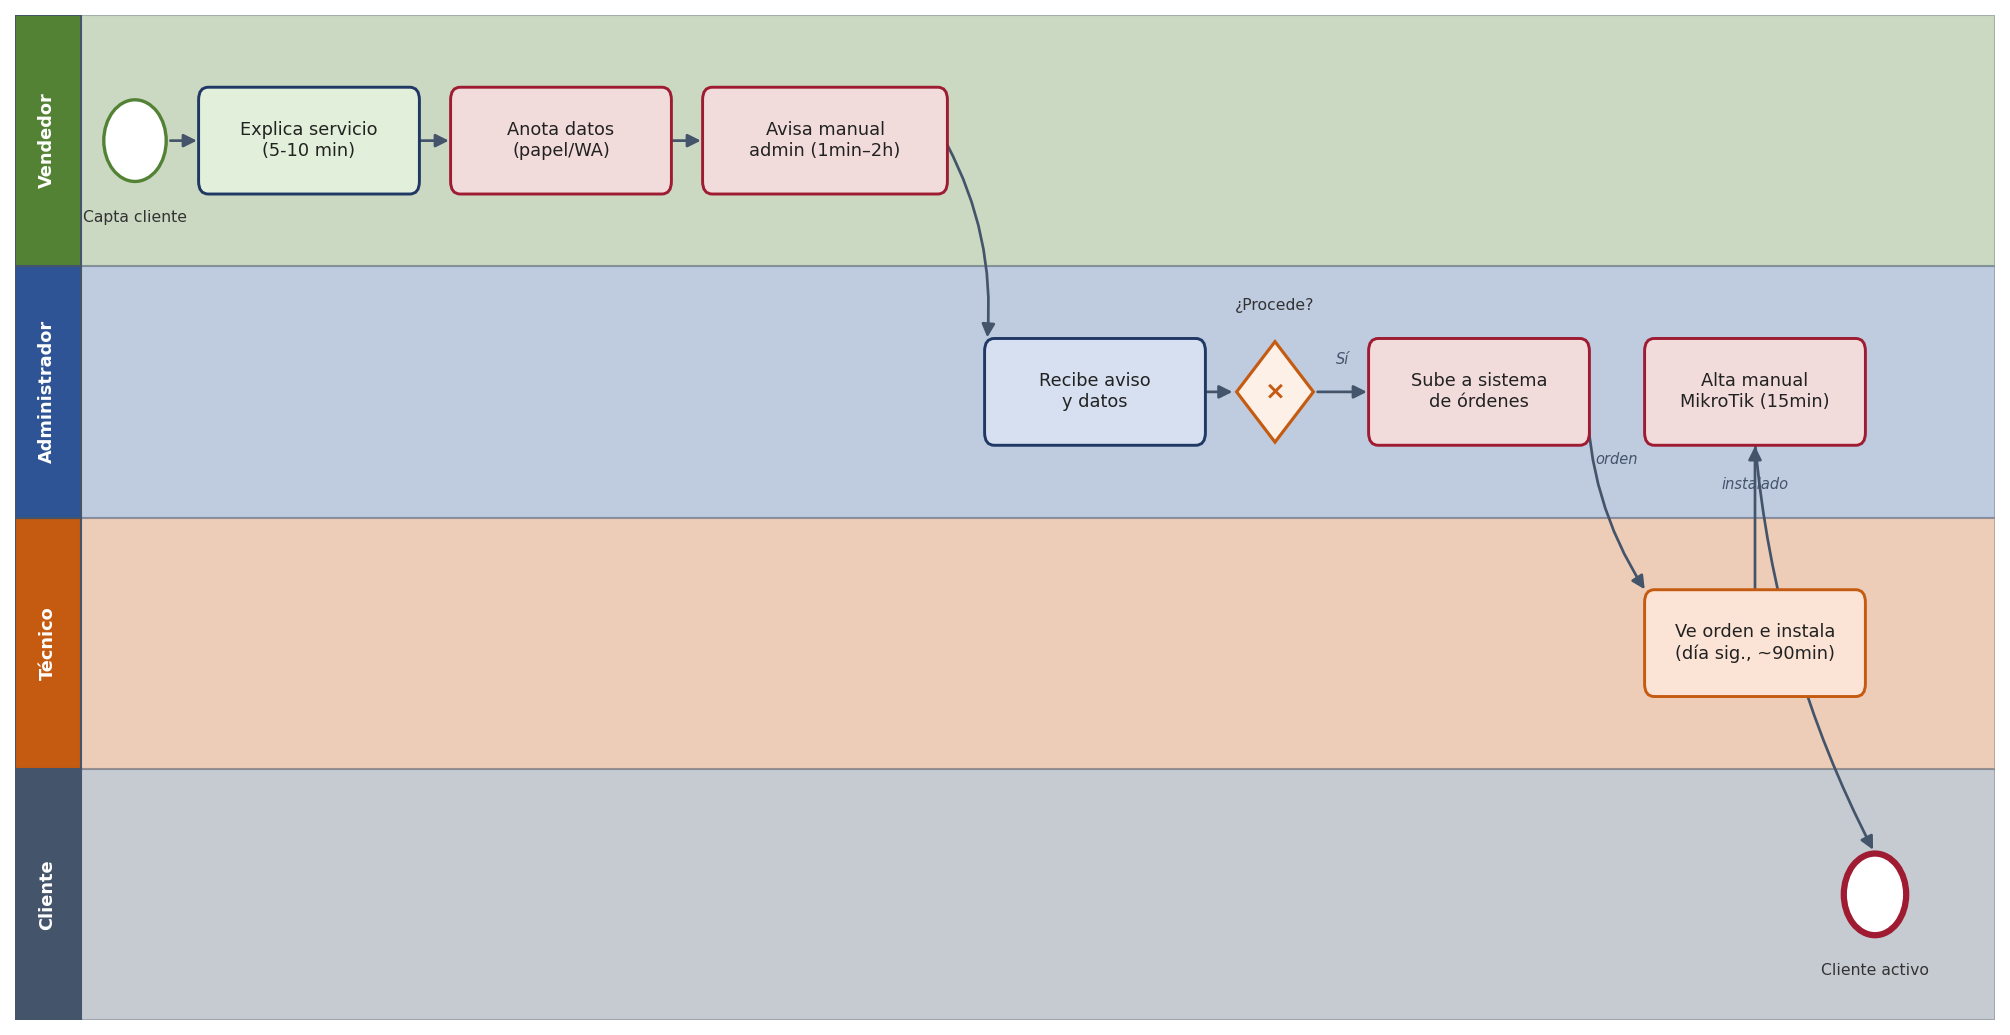
\includegraphics[width=\textwidth]{bpmn_asis.png}
\captionof{figure}{Diagrama BPMN del ciclo de vida del cliente actual (AS-IS). En
rojo, las tareas manuales críticas que generan demoras y pérdidas.}
\label{fig:bpmn-asis}
\end{center}

\subsection{Indicadores actuales (AS-IS)}

A partir de los tiempos reales observados en la operación de WISP, se establecen los
siguientes indicadores del proceso actual:

\begin{center}
\captionof{table}{Indicadores del proceso actual (AS-IS).}
\label{tab:ind-asis}
\begin{tabularx}{\textwidth}{L{4.3cm} L{2.6cm} X}
\toprule
\textbf{Indicador} & \textbf{Valor actual} & \textbf{Observación} \\
\midrule
Tiempo de captación & 5--10 min & Conversación con el prospecto (humano). \\
Tiempo de transferencia al admin & 1 min -- 2 h &
Aviso manual, sin notificación automática. Cuello de botella. \\
Alta manual en MikroTik & $\sim$15 min & El admin entra manualmente a cada MikroTik. \\
Lead time total (captación \textrightarrow{} activación) & $\sim$27 h ($\sim$1.1 días) &
Incluye espera de instalación de un día para otro. \\
Tiempo de trabajo efectivo & $\sim$198 min & Suma de tareas activas (sin esperas). \\
Clientes perdidos en el proceso & 1--2 por ciclo & Prospectos captados que nunca se activan. \\
Trazabilidad de la instalación & 0\% & Evidencias por WhatsApp, sin vínculo al cliente. \\
\bottomrule
\end{tabularx}
\end{center}

\subsection{Problemas detectados}

\begin{itemize}[leftmargin=1.4em]
  \item \textbf{Dependencia del aviso manual:} el proceso se detiene hasta que el
  vendedor logra contactar al administrador; no hay notificaciones automáticas.
  \item \textbf{Pérdida y dispersión de datos:} la información se anota en papel o
  WhatsApp, lo que genera errores de transcripción y prospectos perdidos.
  \item \textbf{Doble digitación:} los datos se registran informalmente y luego el
  admin los reingresa al sistema de órdenes.
  \item \textbf{Alta manual en MikroTik:} el administrador debe ingresar a cada
  router para activar al cliente, tarea repetitiva y propensa a error en 13 zonas.
  \item \textbf{Sin trazabilidad técnica:} las evidencias de instalación (caja NAP,
  borne, equipos) se envían por WhatsApp y no quedan vinculadas al cliente.
  \item \textbf{Cuello de botella en el administrador:} toda la operación depende de
  una sola persona disponible.
\end{itemize}

% ======================================================================
\section{Proceso Propuesto (TO-BE)}
\label{sec:tobe}

\subsection{Rediseño del flujo}

El proceso rediseñado incorpora el sistema de gestión integral como un actor activo
(carril «Sistema») que automatiza las transferencias de información y elimina los
avisos manuales. El vendedor registra al prospecto directamente en la aplicación
móvil, en el momento y lugar de la captación. El sistema valida automáticamente la
cobertura de la zona y notifica de inmediato al administrador, sin que el vendedor
tenga que contactarlo.

El administrador valida el prospecto con un solo clic (los datos ya están
estructurados y disponibles), y el sistema genera automáticamente la orden de
instalación, notificando al técnico en su aplicación. El técnico realiza la
instalación y registra la evidencia (fotos de caja NAP, borne, equipos, fachada)
directamente en la app, vinculada al cliente. Al cerrar la orden, el sistema da de
alta automáticamente al cliente como usuario PPPoE en el MikroTik correspondiente
mediante la API de RouterOS, dejándolo activo de forma inmediata.

\subsection{Diagrama BPMN — Proceso Propuesto (TO-BE)}

\begin{center}
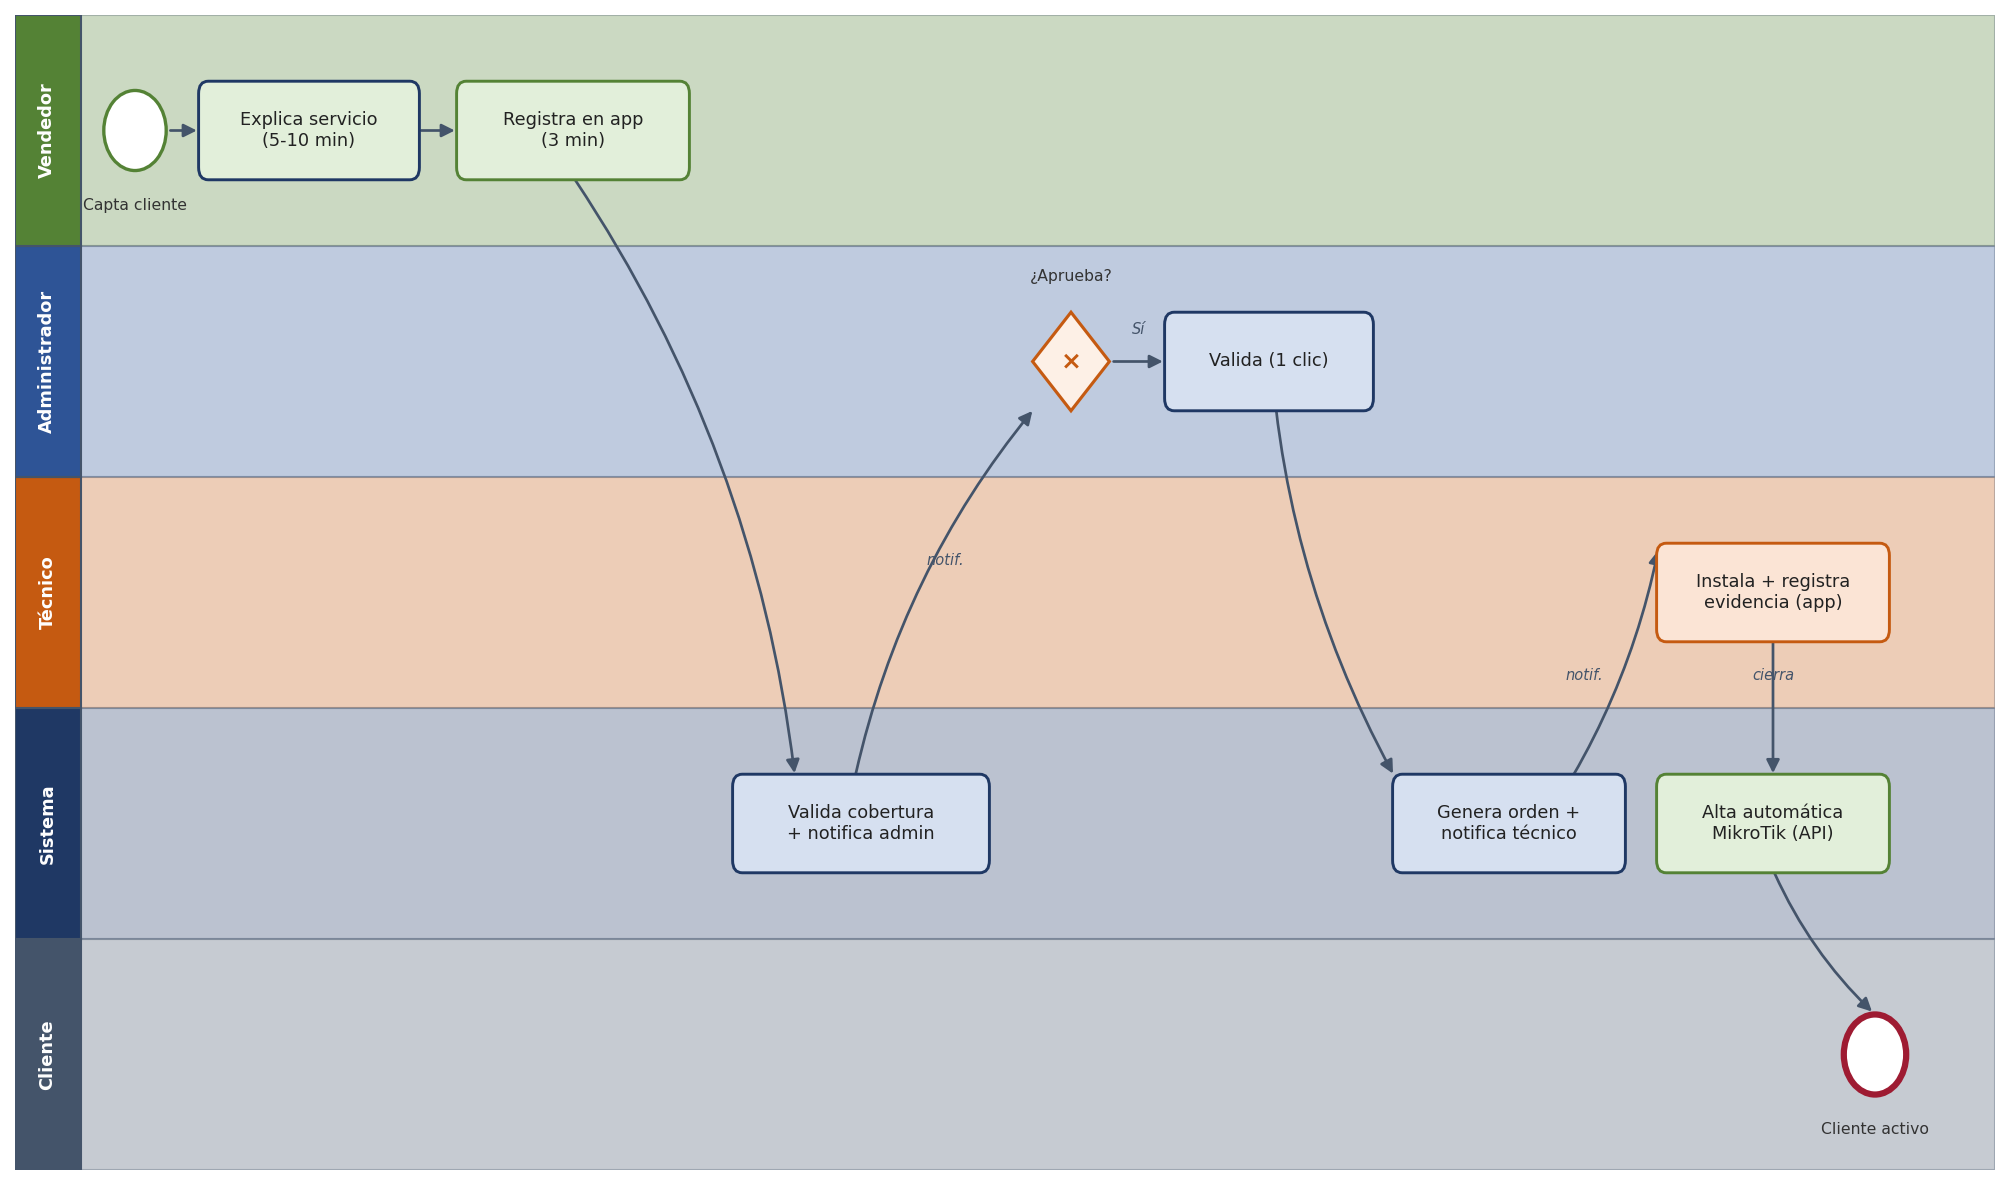
\includegraphics[width=\textwidth]{bpmn_tobe.png}
\captionof{figure}{Diagrama BPMN del ciclo de vida del cliente propuesto (TO-BE). El
carril «Sistema» automatiza validaciones, notificaciones y el alta en MikroTik.}
\label{fig:bpmn-tobe}
\end{center}

\subsection{Automatizaciones propuestas}

El rediseño introduce las siguientes automatizaciones apoyadas en TIC:

\begin{center}
\captionof{table}{Automatizaciones introducidas por el rediseño.}
\label{tab:automatizaciones}
\begin{tabularx}{\textwidth}{L{3.8cm} X L{3.8cm}}
\toprule
\textbf{Automatización} & \textbf{Reemplaza a} & \textbf{Tecnología} \\
\midrule
Registro digital en campo & Anotación en papel/WhatsApp & App móvil (rol vendedor) \\
Notificación automática al admin & Aviso manual (1 min--2 h) & Notificaciones push / backend \\
Validación de cobertura & Verificación mental del admin & Sistema (zonas georreferenciadas) \\
Generación de orden & Subida manual a órdenes & Backend Django \\
Registro de evidencia técnica & Fotos sueltas por WhatsApp & App móvil (rol técnico) \\
Alta automática en MikroTik & Alta manual ($\sim$15 min) & API RouterOS $+$ WireGuard \\
\bottomrule
\end{tabularx}
\end{center}

\subsection{Nuevos indicadores (TO-BE)}

\begin{center}
\captionof{table}{Indicadores del proceso propuesto (TO-BE).}
\label{tab:ind-tobe}
\begin{tabularx}{\textwidth}{L{4.3cm} L{3.2cm} X}
\toprule
\textbf{Indicador} & \textbf{Valor propuesto} & \textbf{Mejora} \\
\midrule
Tiempo de transferencia al admin & Instantáneo ($\sim$0.1 min) & Notificación automática \\
Alta en MikroTik & $\sim$0.5 min (automática) & Vía API RouterOS \\
Lead time total & $\sim$14 h ($\sim$0.6 días) & Mejor coordinación \\
Tiempo de trabajo efectivo & $\sim$111 min & Menos pasos manuales \\
Tiempo de admin por cliente & $\sim$5.5 min & Antes $\sim$86 min \\
Trazabilidad de instalación & 100\% & Evidencia vinculada \\
Clientes perdidos & $\approx$ 0 & Registro inmediato \\
\bottomrule
\end{tabularx}
\end{center}

\begin{upeubox}{Mejora estimada en eficiencia}
El rediseño reduce el tiempo total del ciclo (\textit{lead time}) en aproximadamente
un \textbf{49\%}, el tiempo de trabajo efectivo en un \textbf{44\%}, y el tiempo de
gestión del administrador por cliente en un \textbf{94\%}. El impacto más
significativo se da en la transferencia de información (de hasta 2 horas a
instantánea, una reducción del 96\%) y en el alta en MikroTik (de 15 minutos manuales
a medio minuto automático, un 97\% menos).
\end{upeubox}

% ======================================================================
\section{Análisis Comparativo}
\label{sec:comparativo}

Se comparan cuantitativamente los procesos AS-IS y TO-BE en las tres dimensiones
exigidas: tiempo, costo y calidad.

\subsection{Reducción de tiempos}

\begin{center}
\captionof{table}{Comparación de tiempos entre AS-IS y TO-BE.}
\label{tab:comp-tiempos}
\begin{tabularx}{\textwidth}{L{3.8cm} X X C{1.9cm}}
\toprule
\textbf{Métrica de tiempo} & \textbf{AS-IS} & \textbf{TO-BE} & \textbf{Reducción} \\
\midrule
Transferencia al admin & 1 min--2 h & Instantáneo & 96\% \\
Alta en MikroTik & $\sim$15 min & $\sim$0.5 min & 97\% \\
Trabajo efectivo total & $\sim$198 min & $\sim$111 min & 44\% \\
Lead time (ciclo completo) & $\sim$27 h & $\sim$14 h & 49\% \\
Gestión admin por cliente & $\sim$86 min & $\sim$5.5 min & 94\% \\
\bottomrule
\end{tabularx}
\end{center}

\subsection{Reducción de costos}

La reducción de tiempos se traduce en ahorro de costos operativos, principalmente por
la liberación de tiempo del administrador y la reducción de clientes perdidos:

\begin{center}
\captionof{table}{Comparación de costos entre AS-IS y TO-BE.}
\label{tab:comp-costos}
\begin{tabularx}{\textwidth}{L{4cm} X X X}
\toprule
\textbf{Concepto} & \textbf{AS-IS} & \textbf{TO-BE} & \textbf{Impacto} \\
\midrule
Tiempo admin/cliente valorizado & $\sim$86 min & $\sim$5.5 min & $-$94\% \\
Clientes perdidos por ciclo & 1--2 & $\approx$ 0 & Ingreso recuperado \\
Retrabajo (doble digitación) & Sí & Eliminado & $-$100\% \\
\bottomrule
\end{tabularx}
\end{center}

\textit{Nota:} la valorización económica detallada de estos ahorros se desarrolla en
el Business Case (beneficio de ahorro administrativo y recuperación por menor pérdida
de clientes).

\subsection{Mejora en calidad del servicio}

\begin{center}
\captionof{table}{Comparación de la calidad del servicio entre AS-IS y TO-BE.}
\label{tab:comp-calidad}
\begin{tabularx}{\textwidth}{L{4cm} X X}
\toprule
\textbf{Dimensión de calidad} & \textbf{AS-IS} & \textbf{TO-BE} \\
\midrule
Trazabilidad del cliente & 0\% (WhatsApp/papel) & 100\% en el sistema \\
Historial técnico (NAP, borne, ONU) & Inexistente & Registrado y vinculado \\
Errores de transcripción & Frecuentes & Minimizados (registro directo) \\
Consistencia de datos & Datos dispersos & Fuente única de verdad \\
Experiencia del cliente & Activación variable & Activación más rápida \\
Dependencia de una persona & Total (admin) & Distribuida (sistema) \\
\bottomrule
\end{tabularx}
\end{center}

\begin{upeubox}{Conclusión del análisis comparativo}
El rediseño del proceso (TO-BE) mejora simultáneamente las tres dimensiones: reduce
el tiempo del ciclo en $\sim$49\% y la carga del administrador en $\sim$94\%, elimina
el retrabajo y la pérdida de clientes, y eleva la calidad al garantizar trazabilidad
total, historial técnico y una fuente única de datos. La mejora no es incremental sino
estructural: se pasa de un proceso dependiente de avisos manuales y personas, a un
proceso automatizado, trazable y escalable. Este rediseño constituye la justificación
operativa directa del sistema propuesto.
\end{upeubox}
 % Entregable 4: Modelado de Procesos AS-IS / TO-BE
% ======================================================================
% capitulos/capitulo5.tex
% ----------------------------------------------------------------------
% ENTREGABLE 5 — SOLUCIÓN TIC INTEGRADA al Ecosistema de Sistemas de Información
% Empresa caso de estudio: WISP Ingeniería en Redes y Telecomunicaciones
% Stack: Django · Angular · PostgreSQL · App móvil · WireGuard · API RouterOS
% Contenido trasladado desde Entregable5_SolucionTIC_GTI_WISP.docx
% ======================================================================
\chapter{Solución TIC Integrada al Ecosistema de Sistemas de Información}
\label{chap:soluciontic}

% ----------------------------------------------------------------------
% Descripción del producto (introducción del capítulo)
% ----------------------------------------------------------------------
El presente documento constituye el diseño conceptual y técnico de la solución
tecnológica propuesta para WISP: el \textbf{Sistema de Gestión Integral para ISP de
Fibra Óptica Multi-Zona}. Considera su integración con los sistemas y la
infraestructura existentes, la arquitectura organizacional, los flujos de datos y los
requisitos de seguridad.

Se describe la arquitectura de la solución y sus componentes, el ecosistema de
sistemas de información y su interoperabilidad, los mecanismos de seguridad y
gobernanza (alineados a COBIT 2019 y a la normativa peruana de protección de datos),
y los lineamientos de escalabilidad y sostenibilidad, asegurando la coherencia con el
ecosistema institucional y con los objetivos estratégicos definidos en los
entregables previos.

\begin{upeubox}{Fundamento metodológico: descripción de arquitectura}
La arquitectura se documenta siguiendo el enfoque de vistas del modelo C4 (contexto,
contenedores, componentes) y el estándar ISO/IEC/IEEE~42010 de descripción de
arquitectura, complementados con un modelo de capas (\textit{layered architecture})
para representar la separación de responsabilidades.
\end{upeubox}

% ======================================================================
\section{Arquitectura de la Solución}
\label{sec:arquitectura}

La solución adopta una arquitectura cliente-servidor multicapa, desplegada en la nube
y conectada de forma segura con la infraestructura física distribuida en las 13 zonas
de WISP. El backend centralizado expone una API REST que consumen tanto el frontend
web como la aplicación móvil, y se comunica con los 13 MikroTik a través de una red
privada virtual (WireGuard) usando la API nativa de RouterOS~7.

\subsection{Diagrama de arquitectura (vista de despliegue)}

\begin{center}
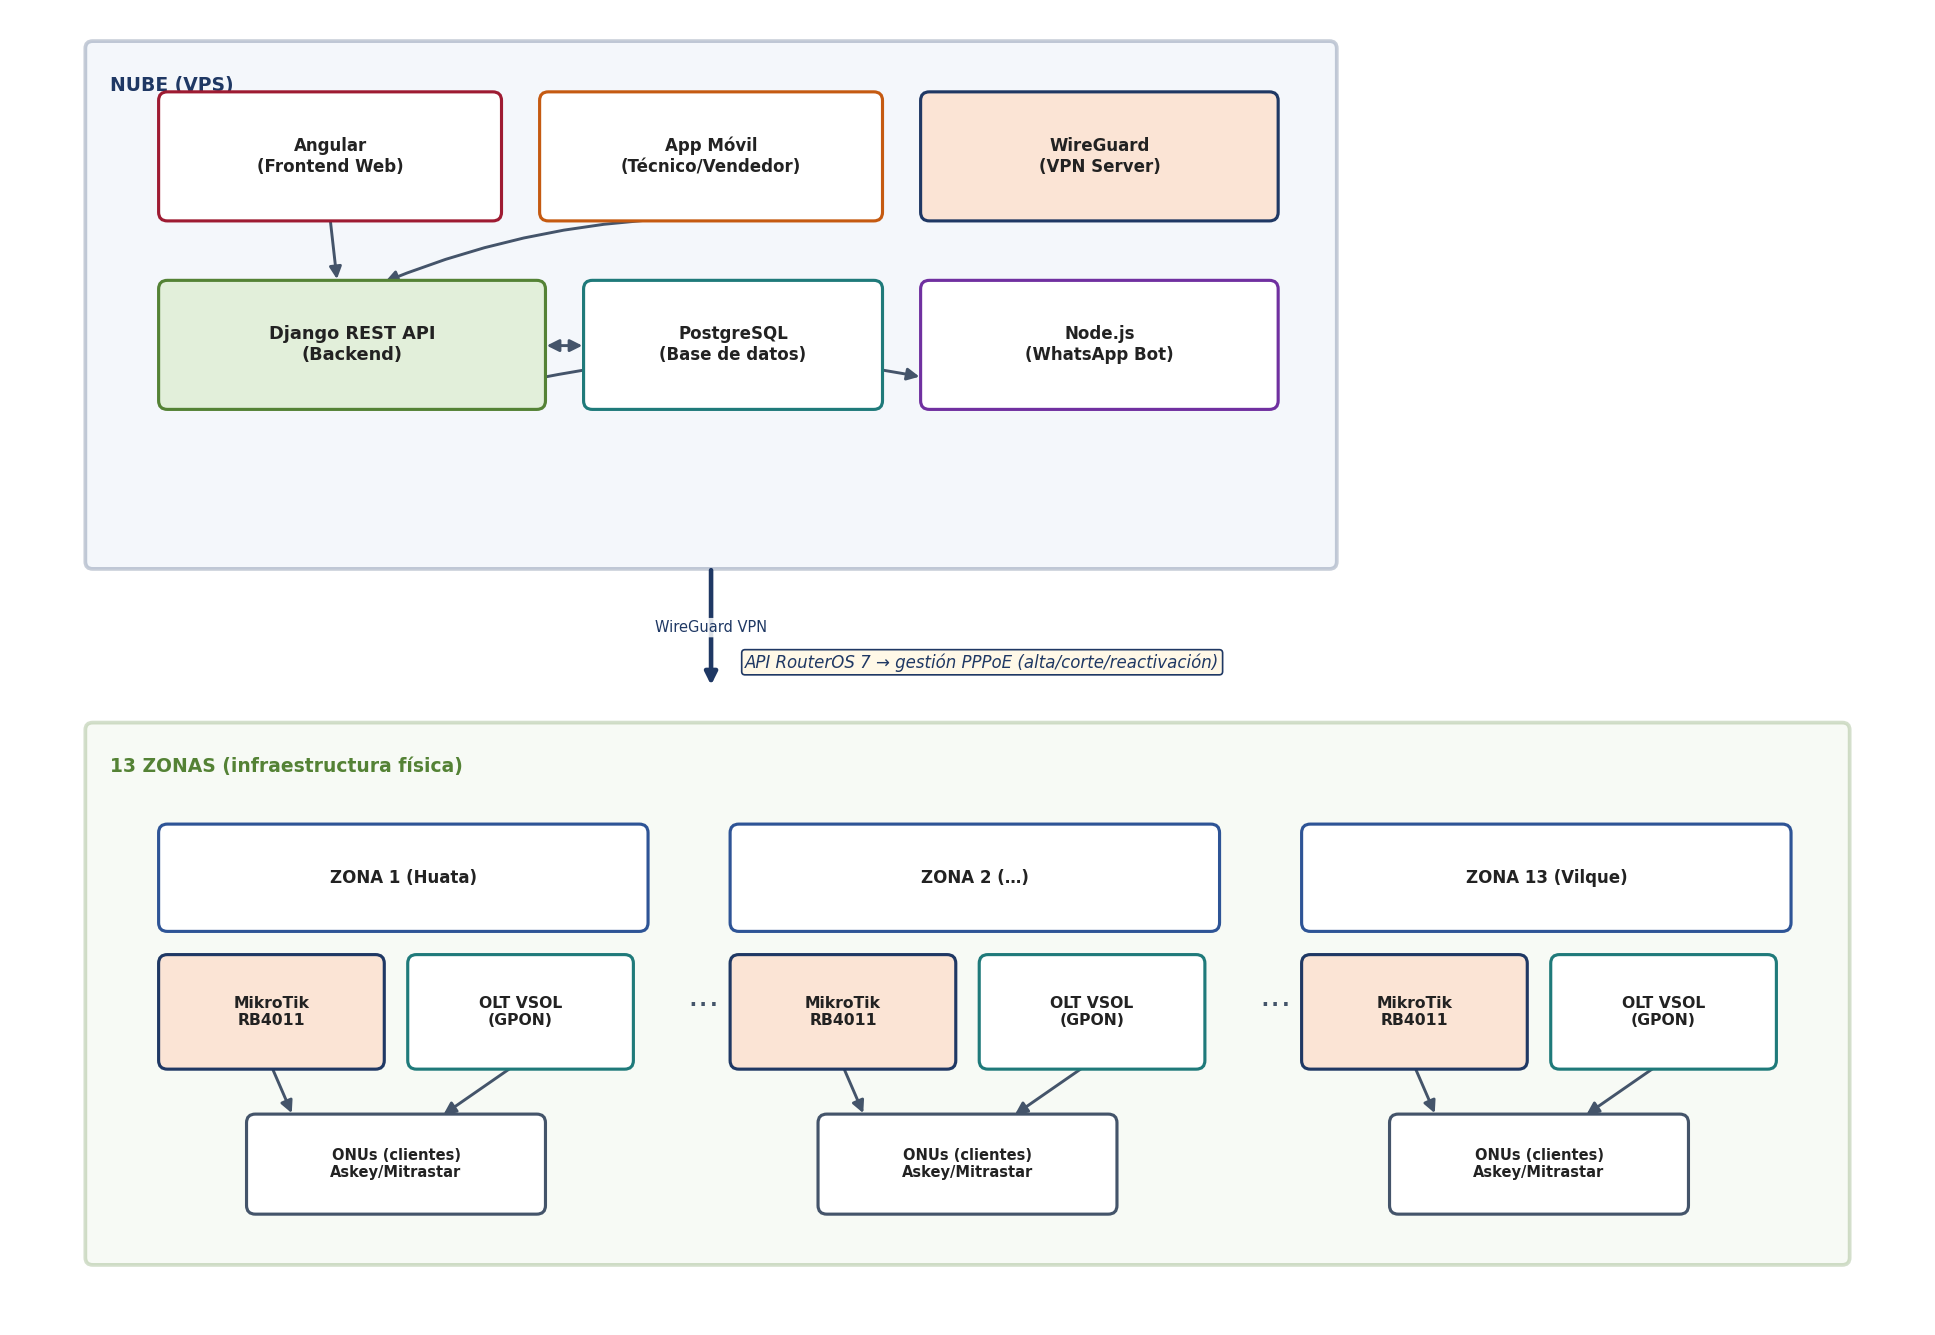
\includegraphics[width=\textwidth]{arq_despliegue.png}
\captionof{figure}{Arquitectura de despliegue: componentes en la nube (VPS) conectados
vía WireGuard con los 13 MikroTik y OLT de cada zona.}
\label{fig:arq-despliegue}
\end{center}

\subsection{Arquitectura por capas}

La solución se organiza en cinco capas con responsabilidades bien separadas, lo que
favorece el mantenimiento, la seguridad y la escalabilidad:

\begin{center}
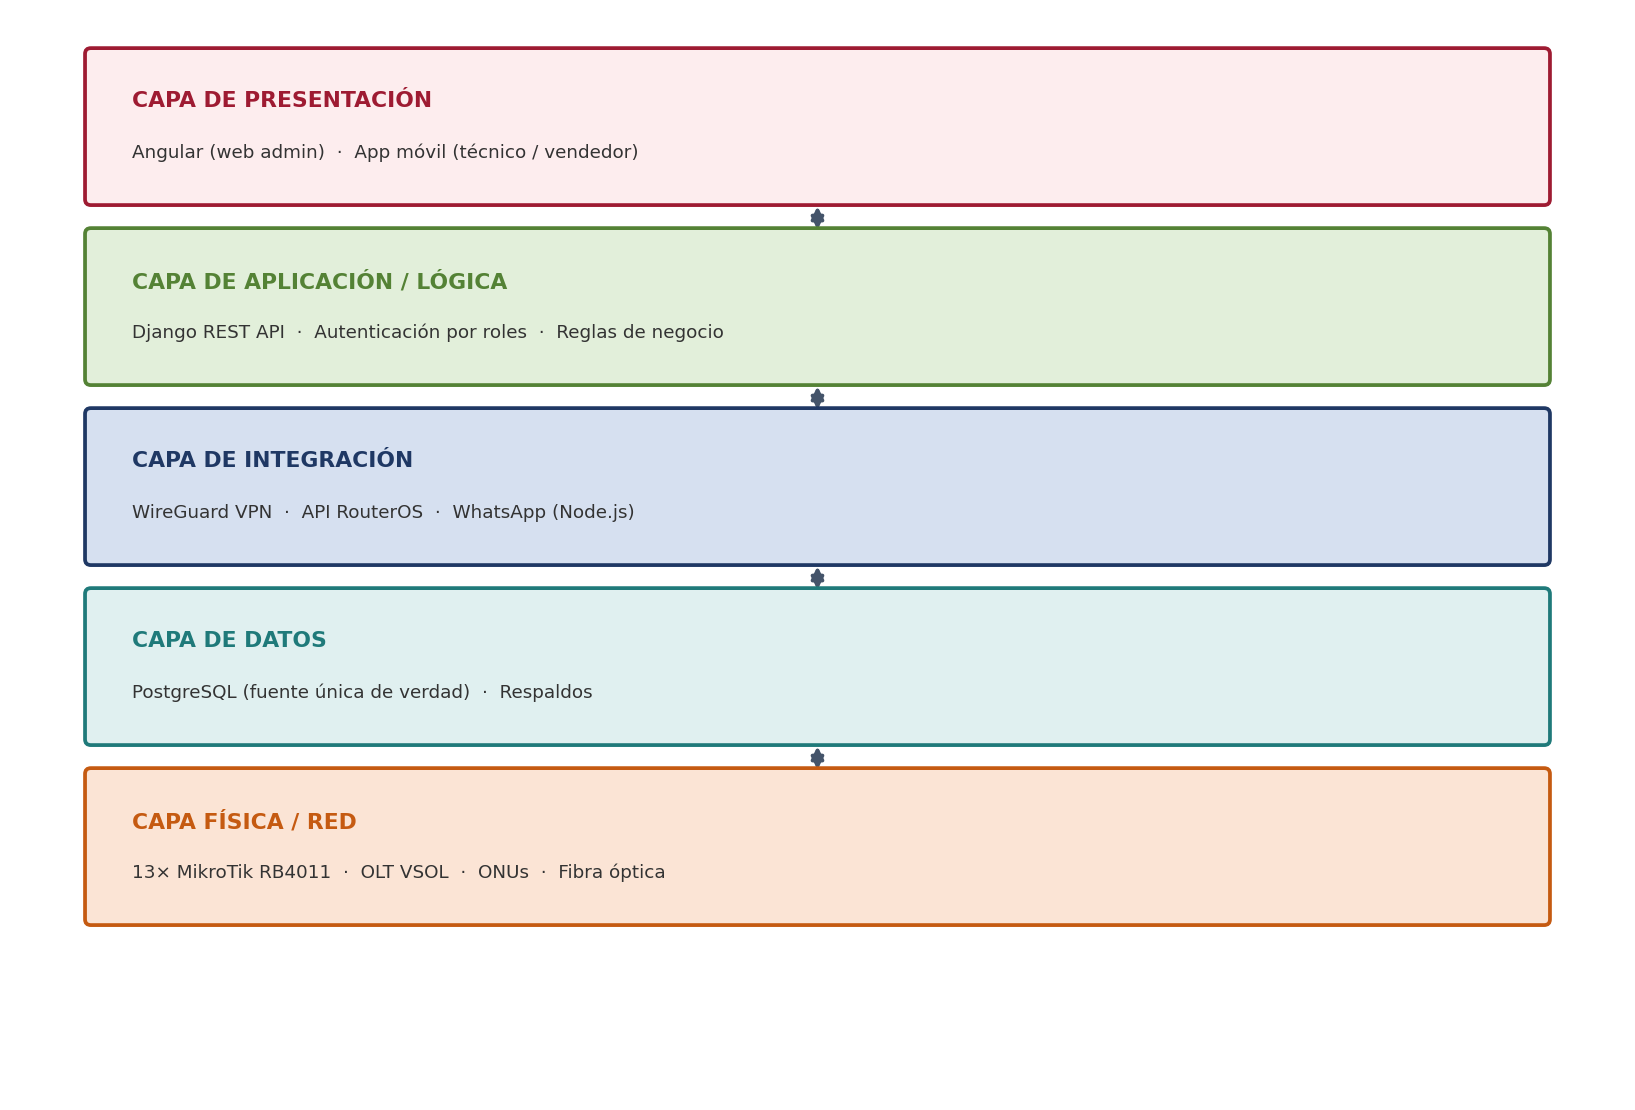
\includegraphics[width=0.9\textwidth]{arq_capas.png}
\captionof{figure}{Arquitectura en capas (\textit{layered architecture}) de la
solución.}
\label{fig:arq-capas}
\end{center}

\subsection{Componentes principales}

\begin{center}
\captionof{table}{Componentes principales de la solución.}
\label{tab:componentes}
\begin{tabularx}{\textwidth}{L{3cm} L{3.2cm} X}
\toprule
\textbf{Componente} & \textbf{Tecnología} & \textbf{Función} \\
\midrule
Frontend web & Angular &
Panel de administración: gestión de clientes, planes, zonas, órdenes y cobertura. \\
Aplicación móvil & App móvil (roles) &
Registro de prospectos (vendedor) y evidencias de instalación (técnico) desde el celular. \\
Backend / API & Django REST Framework &
Lógica de negocio, autenticación por roles, exposición de API REST y orquestación de
integraciones. \\
Base de datos & PostgreSQL &
Fuente única de verdad: clientes, planes, zonas, órdenes, instalaciones, usuarios. \\
VPN & WireGuard &
Túnel cifrado entre la nube y los 13 MikroTik para gestión remota segura. \\
Integración de red & API RouterOS~7 &
Alta, corte y reactivación automática de usuarios PPPoE en los MikroTik. \\
Notificaciones & Node.js (WhatsApp) &
Envío automático de mensajes a clientes (avisos, cobros, estados). \\
\bottomrule
\end{tabularx}
\end{center}

\subsection{Integraciones}

La solución integra tres tipos de sistemas, lo que constituye su principal
diferenciador técnico:

\begin{itemize}[leftmargin=1.4em]
  \item \textbf{Integración con MikroTik (RouterOS API):} el backend crea, corta y
  reactiva usuarios PPPoE y gestiona la lista de corte de morosos directamente en cada
  router, eliminando la operación manual.
  \item \textbf{Integración con WhatsApp (Node.js):} envío automatizado de
  notificaciones a los clientes, reutilizando el canal ya conocido por la empresa.
  \item \textbf{Integración interna (web $+$ móvil $+$ BD):} todos los clientes (web y
  móvil) consumen la misma API y la misma base de datos, garantizando consistencia.
\end{itemize}

% ======================================================================
\section{Ecosistema de Sistemas de Información}
\label{sec:ecosistema}

\subsection{Mapa de sistemas actuales}

El ecosistema actual de WISP está compuesto por sistemas aislados que no se comunican
entre sí, lo que genera la dispersión de datos identificada en el diagnóstico:

\begin{center}
\captionof{table}{Mapa de sistemas actuales y su destino en la solución.}
\label{tab:mapa-sistemas}
\begin{tabularx}{\textwidth}{L{3.6cm} X X}
\toprule
\textbf{Sistema actual} & \textbf{Rol} & \textbf{Destino en la solución} \\
\midrule
Sistema heredado (PHP) & Gestión de clientes & Reemplazado por el nuevo sistema web \\
13$\times$ MikroTik RouterOS~7 & Control PPPoE y ancho de banda & Integrado vía API \\
OLT VSOL ($\times$13) & Concentración de fibra (GPON) & Se mantiene (capa física) \\
Bot WhatsApp (pagos) & Recepción de comprobantes & Coexiste (fuera del alcance actual) \\
WhatsApp operativo & Coordinación informal & Reemplazado por app $+$ notificaciones \\
Papel / registros manuales & Captación en campo & Reemplazado por app móvil \\
\bottomrule
\end{tabularx}
\end{center}

\subsection{Integración propuesta}

La solución actúa como núcleo integrador del ecosistema: centraliza la información
dispersa y se convierte en el punto único de gestión. El sistema heredado y los flujos
de papel/WhatsApp se sustituyen; los MikroTik y OLT (infraestructura física) se
conservan pero pasan a ser gestionados desde el sistema; y el canal WhatsApp se
automatiza. De un ecosistema fragmentado se pasa a un ecosistema integrado alrededor de
una fuente única de verdad.

\begin{upeubox}{Principio de integración adoptado}
Se aplica el principio de «fuente única de verdad» (\textit{single source of truth}):
toda la información operativa reside en la base de datos PostgreSQL, y los distintos
clientes (web, móvil) y sistemas (MikroTik, WhatsApp) se sincronizan con ella. Esto
elimina la duplicidad y las inconsistencias que hoy existen entre el sistema heredado,
los comentarios de los MikroTik y los chats.
\end{upeubox}

\subsection{Interoperabilidad}

La interoperabilidad entre los componentes se garantiza mediante estándares abiertos y
protocolos ampliamente soportados:

\begin{center}
\captionof{table}{Interoperabilidad entre componentes de la solución.}
\label{tab:interoperabilidad}
\begin{tabularx}{\textwidth}{L{3.8cm} X L{3cm}}
\toprule
\textbf{Interacción} & \textbf{Protocolo / Estándar} & \textbf{Formato} \\
\midrule
Web/Móvil $\leftrightarrow$ Backend & HTTP/HTTPS (REST) & JSON \\
Backend $\leftrightarrow$ MikroTik & API REST RouterOS~7 sobre VPN & JSON / HTTPS \\
Nube $\leftrightarrow$ Zonas & WireGuard (UDP cifrado) & Túnel VPN \\
Backend $\leftrightarrow$ WhatsApp & API / librería Node.js & JSON \\
Backend $\leftrightarrow$ Base de datos & SQL / ORM (Django) & Relacional \\
\bottomrule
\end{tabularx}
\end{center}

% ======================================================================
\section{Seguridad y Gobernanza}
\label{sec:seguridad}

La seguridad y la gobernanza de la solución se abordan en dos planos complementarios:
los controles técnicos de seguridad de la información, y el marco de gobierno de TI que
asegura que la tecnología esté alineada con los objetivos de WISP y sea gestionada con
criterios reconocidos.

\begin{upeubox}{Fundamento metodológico: gobierno de TI (COBIT 2019)}
La gobernanza se alinea con COBIT~2019 (ISACA), marco de referencia para el gobierno y
la gestión de la tecnología de la información empresarial. Se referencian objetivos de
gobierno y gestión (\textit{governance/management objectives}) aplicables a la
solución. Esto responde al lineamiento de «Gobierno de TI» que el propio programa de
GTI establece para el área.
\end{upeubox}

\subsection{Gestión de accesos}

El control de accesos se basa en el principio de mínimo privilegio y en la autenticación
por roles (RBAC --- \textit{Role-Based Access Control}), de modo que cada usuario accede
únicamente a las funciones que su rol requiere:

\begin{center}
\captionof{table}{Control de accesos por rol (RBAC).}
\label{tab:accesos}
\begin{tabularx}{\textwidth}{L{2.6cm} X L{3.6cm}}
\toprule
\textbf{Rol} & \textbf{Accesos permitidos} & \textbf{Restricciones} \\
\midrule
Administrador &
Gestión completa: clientes, planes, zonas, órdenes, cortes, reportes. &
Acceso total (supervisado) \\
Vendedor &
Registro de prospectos y consulta de cobertura desde la app. &
No accede a datos de red ni cortes \\
Técnico &
Órdenes asignadas y registro de evidencias de instalación. &
No accede a datos comerciales/financieros \\
Cliente (futuro) &
Consulta de su estado y cobertura (autoservicio). &
Solo su propia información \\
\bottomrule
\end{tabularx}
\end{center}

\subsection{Protección de datos}

La protección de los datos ---especialmente los datos personales de los clientes--- se
garantiza mediante los siguientes controles técnicos:

\begin{itemize}[leftmargin=1.4em]
  \item \textbf{Cifrado en tránsito:} todo el tráfico web usa HTTPS/TLS, y la
  comunicación con los MikroTik viaja por el túnel cifrado WireGuard.
  \item \textbf{Autenticación robusta:} credenciales protegidas (\textit{hashing}),
  tokens de sesión y control por roles.
  \item \textbf{Respaldos periódicos:} copias de seguridad automáticas de la base de
  datos, con plan de recuperación.
  \item \textbf{Registro de auditoría:} trazabilidad de las acciones críticas (altas,
  cortes, cambios) para responsabilidad y control.
  \item \textbf{Segmentación de red:} acceso a los MikroTik restringido a través de la
  VPN, sin exposición directa a internet.
\end{itemize}

\subsection{Cumplimiento normativo}

La solución se diseña considerando el marco legal peruano y las buenas prácticas del
sector:

\begin{center}
\captionof{table}{Marco normativo aplicable a la solución.}
\label{tab:normativo}
\begin{tabularx}{\textwidth}{L{3cm} L{3.4cm} X}
\toprule
\textbf{Norma / Marco} & \textbf{Ámbito} & \textbf{Aplicación en la solución} \\
\midrule
Ley N° 29733 & Protección de Datos Personales (Perú) &
Tratamiento seguro y consentido de los datos de clientes. \\
OSIPTEL / MTC & Regulación de telecomunicaciones &
Registro ordenado de clientes y servicios prestados. \\
ISO/IEC 27001 (ref.) & Seguridad de la información &
Buenas prácticas de controles de seguridad. \\
COBIT 2019 & Gobierno y gestión de TI &
Alineamiento estratégico y gestión de riesgos (ver abajo). \\
\bottomrule
\end{tabularx}
\end{center}

\subsection{Gobernanza de TI con COBIT 2019}

Se referencian los objetivos de gobierno y gestión de COBIT~2019 que la solución ayuda
a cumplir, evidenciando que el proyecto no solo construye tecnología, sino que la
gobierna de forma alineada al negocio:

\begin{center}
\captionof{table}{Objetivos de COBIT~2019 cubiertos por la solución.}
\label{tab:cobit}
\begin{tabularx}{\textwidth}{L{3.4cm} L{3.6cm} X}
\toprule
\textbf{Objetivo COBIT 2019} & \textbf{Dominio} & \textbf{Contribución de la solución} \\
\midrule
EDM01 -- Gobierno de TI & Evaluar, Orientar y Supervisar &
La solución alinea la TI con los objetivos estratégicos de WISP definidos en el
diagnóstico. \\
EDM03 -- Optimización del riesgo & Evaluar, Orientar y Supervisar &
Reduce riesgos operativos (dependencia de una persona, pérdida de datos). \\
APO12 -- Gestión del riesgo & Alinear, Planificar y Organizar &
Se apoya en el plan de riesgos del proyecto (análisis P$\times$I y respuestas). \\
APO13 -- Gestión de la seguridad & Alinear, Planificar y Organizar &
Define políticas de seguridad, cifrado y control de accesos. \\
BAI03 -- Gestión de soluciones & Construir, Adquirir e Implementar &
Desarrollo estructurado del sistema (SRS, arquitectura, pruebas). \\
DSS05 -- Servicios de seguridad & Entregar, Dar Servicio y Soporte &
Gestión de accesos por roles, protección de \textit{endpoints} y VPN. \\
\bottomrule
\end{tabularx}
\end{center}

\begin{upeubox}{Lectura de gobernanza}
Al mapear la solución contra COBIT~2019, WISP no solo obtiene un sistema, sino un
modelo de gobierno de su TI: la tecnología queda alineada con la estrategia (EDM01),
los riesgos se gestionan (EDM03, APO12), la seguridad se formaliza (APO13, DSS05) y el
desarrollo sigue buenas prácticas (BAI03). Esto eleva la madurez digital de la empresa
desde el nivel «inicial» diagnosticado hacia un nivel «gestionado».
\end{upeubox}

% ======================================================================
\section{Escalabilidad y Sostenibilidad}
\label{sec:escalabilidad}

\subsection{Capacidad de crecimiento}

La arquitectura está diseñada para crecer sin rediseños estructurales, acompañando la
expansión de WISP a nuevos distritos (objetivo estratégico OE-01):

\begin{itemize}[leftmargin=1.4em]
  \item \textbf{Escalabilidad horizontal de zonas:} agregar una nueva zona solo
  requiere sumar su MikroTik a la VPN y registrarlo; el sistema ya está preparado para
  $N$ zonas, no está limitado a 13.
  \item \textbf{Escalabilidad de usuarios:} el backend Django y PostgreSQL soportan el
  crecimiento de clientes; ante mayor carga, el VPS puede escalar verticalmente (más
  recursos) u horizontalmente (más instancias).
  \item \textbf{Homogeneidad de la infraestructura:} al ser todos los MikroTik del
  mismo modelo y versión (RB4011, RouterOS~7), la integración escala sin casos
  particulares.
  \item \textbf{Arquitectura desacoplada:} la separación en capas y el uso de API
  permiten evolucionar cada componente de forma independiente.
\end{itemize}

\subsection{Costos futuros}

La sostenibilidad económica se sustenta en costos operativos bajos y predecibles, que
crecen mucho más lento que los ingresos por nuevos clientes:

\begin{center}
\captionof{table}{Proyección de costos operativos según escenario de crecimiento.}
\label{tab:costos-futuros}
\begin{tabularx}{\textwidth}{L{4.2cm} L{3.4cm} X}
\toprule
\textbf{Escenario} & \textbf{Costo operativo anual} & \textbf{Observación} \\
\midrule
Actual ($\sim$455 clientes, 13 zonas) & $\sim$S/~3\,780 &
VPS $+$ dominio $+$ mantenimiento $+$ backup \\
Crecimiento ($+$50\% clientes) & $\sim$S/~4\,500--5\,500 &
Solo escala el VPS; el resto se mantiene \\
Nuevas zonas ($+$5 zonas) & Costo marginal bajo &
Sin nuevo desarrollo; solo configuración \\
\bottomrule
\end{tabularx}
\end{center}

\begin{upeubox}{Sostenibilidad económica}
El costo operativo por cliente disminuye a medida que WISP crece (economía de escala):
la misma plataforma soporta más clientes y zonas con un incremento de costo marginal.
Esto hace que la solución sea sostenible en el tiempo y refuerza el retorno demostrado
en el Business Case.
\end{upeubox}

\subsection{Evolución tecnológica}

La solución contempla una hoja de ruta de evolución que aprovecha su arquitectura
desacoplada para incorporar mejoras futuras sin rehacer lo existente:

\begin{center}
\captionof{table}{Hoja de ruta de evolución tecnológica.}
\label{tab:evolucion}
\begin{tabularx}{\textwidth}{L{2.8cm} X L{2.4cm}}
\toprule
\textbf{Fase} & \textbf{Evolución propuesta} & \textbf{Horizonte} \\
\midrule
Corto plazo &
Automatización del módulo de pagos (Yape/Plin) e integración con el bot de cobros. &
6--12 meses \\
Mediano plazo &
Portal de autoservicio para clientes y provisión automática de ONUs en la OLT. &
1--2 años \\
Largo plazo &
Analítica de datos e indicadores de negocio (BI); alertas predictivas de red. &
2$+$ años \\
\bottomrule
\end{tabularx}
\end{center}

% ======================================================================
\section{Conclusión — Cierre de la Línea GTI}
\label{sec:cierre-gti}

La Solución TIC Integrada propuesta constituye una respuesta coherente, técnicamente
sólida y estratégicamente alineada al problema de WISP. Su arquitectura multicapa en la
nube, integrada de forma segura con los 13 MikroTik mediante WireGuard y la API de
RouterOS, convierte un ecosistema hoy fragmentado en una plataforma única, trazable y
escalable.

Con este documento se cierra la línea de Gestión de Tecnologías de Información (GTI),
que ha recorrido de forma completa el ciclo: el diagnóstico organizacional identificó el
problema; el Business Case demostró su viabilidad económica; el Plan de Gestión
estableció cómo ejecutarlo; el modelado de procesos AS-IS/TO-BE cuantificó la mejora
operativa; y esta Solución TIC define el cómo técnico. En conjunto, GTI entrega el marco
estratégico y de gobierno sobre el cual las líneas de Software e Infraestructura
desarrollarán la implementación.

\begin{upeubox}{Coherencia integral del proyecto}
Los cinco componentes de GTI conforman una narrativa única y trazable: problema
\textrightarrow{} viabilidad \textrightarrow{} plan \textrightarrow{} procesos
\textrightarrow{} solución. Cada decisión técnica de esta Solución TIC responde a una
necesidad identificada en el diagnóstico y validada en el Business Case, y se gobierna
con criterios reconocidos (PMBOK, BPMN, COBIT~2019). El proyecto queda listo para su
fase de construcción en las líneas de Software e Infraestructura.
\end{upeubox}
 % Entregable 5: Solución TIC Integrada al Ecosistema de Sistemas de Información

% ====================== LÍNEA CE02 · INGENIERÍA DE SOFTWARE ======================
\part{Línea CE02 — Ingeniería de Software}
% ======================================================================
% capitulos/ce02_ingenieria_software.tex
% ----------------------------------------------------------------------
% LÍNEA CE02 — INGENIERÍA DE SOFTWARE
% Esqueleto / marcador de posición. Reemplazar por los capítulos reales
% conforme se desarrollen los entregables de esta línea.
% ======================================================================
\chapter{Ingeniería de Software — Presentación de la línea}
\label{chap:ce02-intro}

Esta línea (CE02) desarrolla la especificación, el diseño y la construcción del
software del \textbf{Sistema de Gestión Integral para ISP de Fibra Óptica
Multi-Zona}. Toma como insumo los entregables de la línea CE01 (en especial el
\hyperref[chap:procesos]{modelado de procesos (TO-BE)} y la
\hyperref[chap:soluciontic]{solución TIC}) y produce los artefactos de ingeniería
que hacen construible el sistema.

\begin{upeubox}{Entregables planificados de la línea CE02 (en desarrollo)}
Según la EDT del \hyperref[chap:plangestion]{Plan de Gestión}, esta línea comprende:
\begin{itemize}[leftmargin=1.4em]
  \item \textbf{Especificación de requisitos (SRS):} requerimientos funcionales y no
  funcionales conforme a IEEE~29148.
  \item \textbf{Prototipos navegables:} diseño de interfaz (Figma) validado con WISP.
  \item \textbf{Arquitectura de software:} vistas C4 e IEEE/IEEE~42010, y modelado
  UML (casos de uso, clases, secuencia, despliegue).
  \item \textbf{Diseño de base de datos:} modelo entidad-relación, modelo lógico,
  diccionario de datos y scripts SQL (DDL/DML).
  \item \textbf{Construcción del sistema (semestre 2):} backend Django (API REST),
  frontend web Angular, app móvil e integración MikroTik.
\end{itemize}
\end{upeubox}

\medskip
\textit{Nota: los capítulos de esta línea se incorporarán aquí a medida que se
completen sus entregables. Este archivo es un marcador de posición para mantener
integrada la estructura de las tres líneas del proyecto.}

% Al desarrollar, sustituir este archivo (o añadir \input adicionales en main.tex)
% por capítulos como:
%   \input{capitulos/ce02_srs}
%   \input{capitulos/ce02_prototipos}
%   \input{capitulos/ce02_arquitectura_uml}
%   \input{capitulos/ce02_base_datos}
%   \input{capitulos/ce02_construccion}
 % (en desarrollo) SRS, prototipos, arquitectura/UML, base de datos, construcción

% ====================== LÍNEA CE03 · INFRAESTRUCTURA TECNOLÓGICA ======================
\part{Línea CE03 — Infraestructura Tecnológica}
% ======================================================================
% capitulos/ce03_infraestructura.tex
% ----------------------------------------------------------------------
% LÍNEA CE03 — INFRAESTRUCTURA TECNOLÓGICA
% Esqueleto / marcador de posición. Reemplazar por los capítulos reales
% conforme se desarrollen los entregables de esta línea.
% ======================================================================
\chapter{Infraestructura Tecnológica — Presentación de la línea}
\label{chap:ce03-intro}

Esta línea (CE03) define la infraestructura de red y de despliegue que soporta el
sistema: la red de fibra óptica multi-zona de WISP, la interconexión de las 13 zonas
y el entorno donde se ejecuta la solución de software (línea CE02). Se apoya en la
\hyperref[chap:soluciontic]{solución TIC} definida en la línea CE01.

\begin{upeubox}{Entregables planificados de la línea CE03 (en desarrollo)}
El alcance previsto para esta línea comprende:
\begin{itemize}[leftmargin=1.4em]
  \item \textbf{Diseño de la topología de red:} arquitectura multi-zona (OLT, ONU,
  NAP, enlaces de fibra) y diagrama físico y lógico.
  \item \textbf{Direccionamiento y segmentación:} plan de direccionamiento IP, VLAN
  y separación de tráfico por zona/servicio.
  \item \textbf{Equipamiento y configuración:} routers MikroTik RB4011 (RouterOS~7),
  OLT/ONU y parámetros PPPoE.
  \item \textbf{Interconexión y acceso remoto:} VPN WireGuard para gestión
  centralizada de los 13 MikroTik desde el sistema.
  \item \textbf{Seguridad de red:} \textit{hardening}, control de accesos, firewall y
  buenas prácticas.
  \item \textbf{Monitoreo y gestión:} disponibilidad, SNMP y tableros de control de la
  red.
\end{itemize}
\end{upeubox}

\medskip
\textit{Nota: los capítulos de esta línea se incorporarán aquí a medida que se
completen sus entregables. Este archivo es un marcador de posición para mantener
integrada la estructura de las tres líneas del proyecto.}

% Al desarrollar, sustituir este archivo (o añadir \input adicionales en main.tex)
% por capítulos como:
%   \input{capitulos/ce03_topologia}
%   \input{capitulos/ce03_direccionamiento}
%   \input{capitulos/ce03_equipamiento}
%   \input{capitulos/ce03_vpn_interconexion}
%   \input{capitulos/ce03_seguridad}
%   \input{capitulos/ce03_monitoreo}
 % (en desarrollo) diseño de red, direccionamiento, equipamiento, VPN, seguridad, monitoreo

\end{document}
  